\documentclass[xcolor=pdftex,table,10pt,yellow,mathserif]{beamer}
%\usepackage[numbers]{natbib}
\usepackage{array}
\usepackage{amsmath}
\usepackage{ulem}
\usepackage{algorithm,algorithmic}
\usepackage{tikz}
\usepackage{pgflibraryshapes}
\usepackage{beamerthemesplit}
\mode<presentation> {
\usetheme{PSI}
}
\usepackage[english]{babel}
\usetikzlibrary{shapes,arrows,snakes,backgrounds}
\usepackage[overlay,absolute]{textpos}
\usepackage[latin1]{inputenc}
\usepackage{pgfpages}
\usepackage{ulem}
\usetikzlibrary{mindmap,trees}
\usepackage{verbatim}
\usepackage{pgfpages}
\usepackage{bbding}
\xdefinecolor{mygreen}{RGB}{0,220,0}
\xdefinecolor{myblue}{RGB}{26,150,255}

% My own packages... 
\usepackage{comment}
\usepackage{physics} % everyone should use this ;)
% \usepackage{minipage}
\usepackage[style=numeric, backend=biber]{biblatex}
\bibliography{literature.bib}
\renewcommand*{\bibfont}{\tiny} % use tiny font in references!
\nocite{*} % always cite everything
\usepackage{siunitx} % Nice units :)
\usepackage{listings}
\definecolor{codegreen}{rgb}{0,0.6,0}
\definecolor{codegray}{rgb}{0.5,0.5,0.5}
\definecolor{codepurple}{rgb}{0.58,0,0.82}
\definecolor{backcolour}{rgb}{0.95,0.95,0.92}
\lstdefinestyle{mystyle}{
    backgroundcolor=\color{backcolour},   
    commentstyle=\color{codegreen},
    keywordstyle=\color{magenta},
    numberstyle=\tiny\color{codegray},
    stringstyle=\color{codepurple},
    breakatwhitespace=false,     
    basicstyle=\ttfamily\tiny,
    breaklines=true,                 
    captionpos=b,                    
    keepspaces=true,                 
    numbers=left,                    
    numbersep=5pt,                  
    showspaces=false,                
    showstringspaces=false,
    showtabs=false,                  
    tabsize=2
}
\lstset{style=mystyle}



\newcommand{\qvec}{\mathbf{q}}
\newcommand{\lieoperator}[1]{{:\!#1\!:\!}}
%\newcommand{\poissonbracket}[1]{ \left[ #1 \right] }
\newcommand{\lietransformation}[1]{e^{:\!#1\!:}}

\newcommand*\tick{\item[\color{mygreen}\Checkmark]}


\newtheorem{thm}{Theorem}

% ************************ space ************************************
\newcommand{\hhs}[1]{\hspace{#1mm}}
\newcommand{\hs}{\hspace{5mm}}
\newcommand{\vp}{\vspace{1mm}}
\newcommand{\vs}{\vspace{5mm}}
\newcommand{\jl}{$\frac{}{}$} %User defined for empty symbol to jump line
% ********************** newcommand *********************************
\newcommand{\mbf}[1]{\mbox{\boldmath $#1$}}
\newcommand{\hb}[1]{\hspace{-#1 mm}}
\newcommand{\ds}{\displaystyle}
\newcommand{\QED}{\hfill $\Box$}
% *********************** frequently used math symbols from AMS *******
%\newcommand{\norm}[1]{\left\Vert#1\right\Vert}
%\newcommand{\abs}[1]{\left\vert#1\right\vert}
%\newcommand{\set}[1]{\left\{#1\right\}}


\definecolor{Maroon}{rgb}{.5,.1,.25}% Used for Trinity University






\mode<presentation>
{
  \usepackage{pgf}
  \usepackage{hyperref}
  \setbeamercovered{transparent}
  \setbeamercovered{transparent}  
}

\AtBeginSection[]
{
  \begin{frame}<beamer>
    \frametitle{Outline}
    \tableofcontents[currentsection,hideothersubsections]
  \end{frame}
}

\AtBeginSubsection[]
{
  \begin{frame}<beamer>
    \frametitle{Outline}
    \tableofcontents[currentsection,currentsubsection]
  \end{frame}
}


\setbeamercolor{uppercolgreen}{fg=white,bg=yellow!35}
\setbeamercolor{lowercolgreen}{fg=black,bg=yellow!90}


\title{Monte Carlo Solution to Coulomb Collisions}

\author{\href{mailto:alexander.liemen@inf.ethz.ch}{Alexander Liemen}}


\date{\today}

\titlegraphic{
 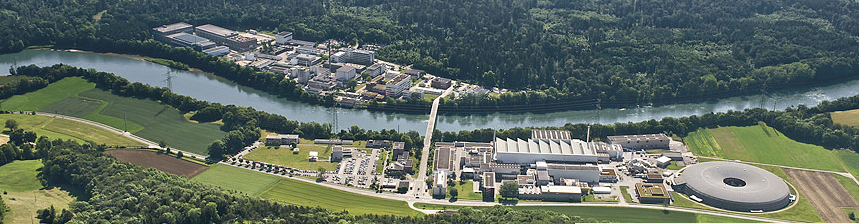
\includegraphics[width=10cm]{./figures/figures-slides/PSI} \\
}

\begin{document}

 \frame{
 \maketitle
}
%
 \frame{
 \tableofcontents
}


% Make the doc cleaner... 

\section{Problem Introduction}

\begin{frame}{} % Project Goal: Charged Particle Cloud Simulation
    \begin{block}{Simulate Relaxation Behaviour of a Charged Particle Cloud}
        Particle characteristics:
        \begin{itemize}
            \item Equal mass and charge
            \item No "physical radius"
            \item Focus on \textsc{Coulomb} interactions
        \end{itemize}
        Collision implementation:
        \begin{itemize}
            \item Direct-Simulation-Monte-Carlo (DSMC) approach
        \end{itemize}
        Flexibility of the algorithm:
        \begin{itemize}
            \item Mass and charge saved individually per particle
            \item Suitable for mixed plasmas (e.g. ion-electron interactions)
        \end{itemize}
    \end{block}
    \begin{minipage}[c]{\textwidth}
        \centering
        \begin{minipage}{0.25\textwidth}
            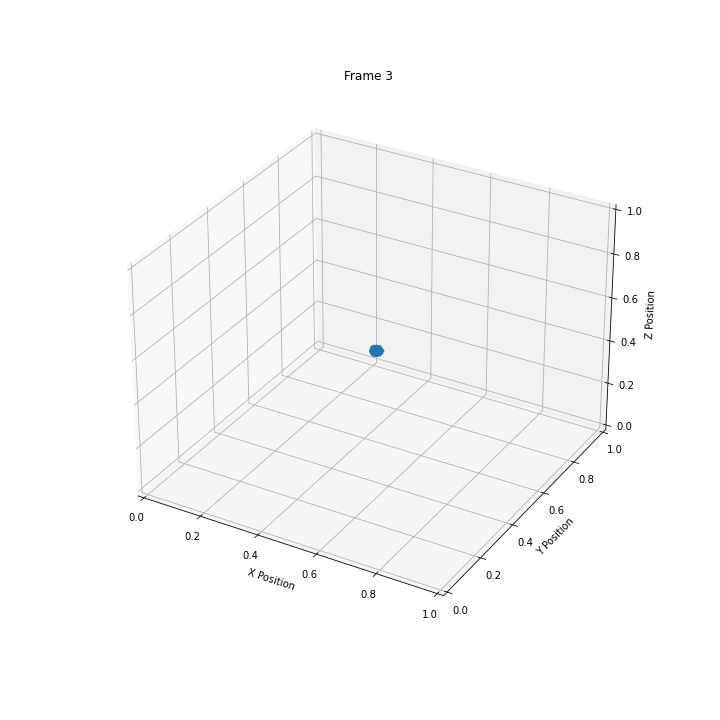
\includegraphics[width=\textwidth]{ressources/particle_expansion/position_2.png}
        \end{minipage}
        $\longrightarrow$
        \begin{minipage}{0.25\textwidth}
            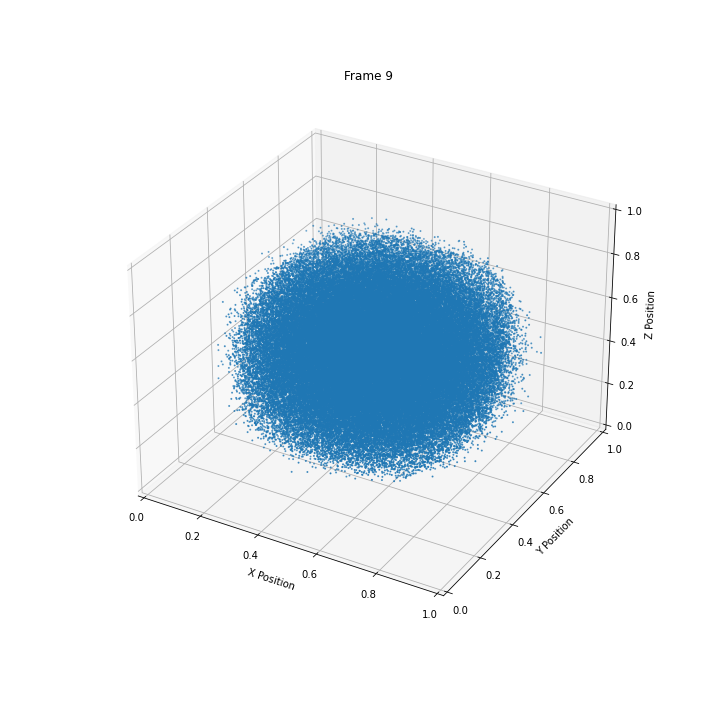
\includegraphics[width=\textwidth]{ressources/particle_expansion/position_8}
        \end{minipage}
        $\longrightarrow$
        \begin{minipage}{0.25\textwidth}
            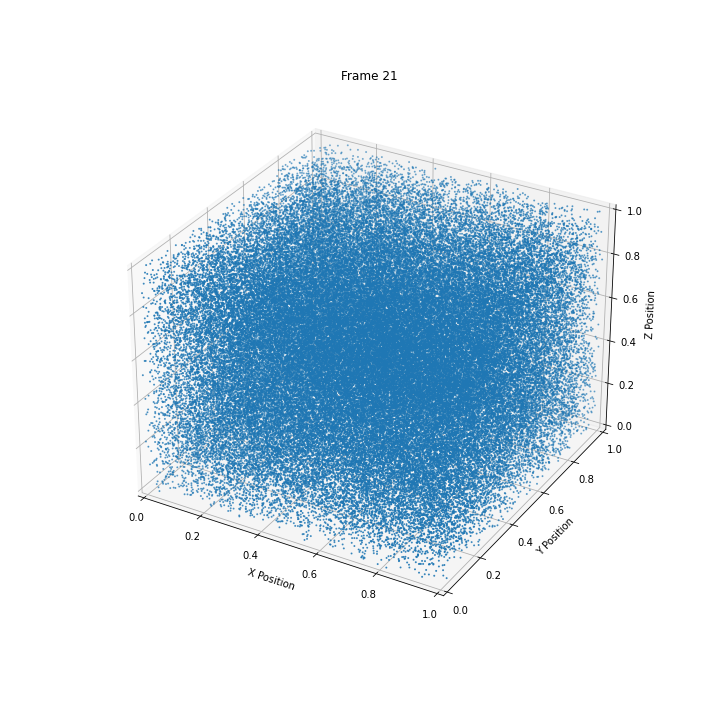
\includegraphics[width=\textwidth]{ressources/particle_expansion/position_20}
        \end{minipage}
    \end{minipage}
\end{frame}

\begin{frame}{Landau-Fokker-Planck}
    Both algorithms converge to the \textsc{Landau-Fokker-Planck} equation.
    \begin{itemize}
        \item \textsc{Boltzmann} equation \cite[1]{Rosenbluth1957} (total force field $F^\mu$):
        \begin{equation*}
            \pdv{f_a}{t} + v^\mu \pdv{f_a}{x^\mu} + \frac{F^\mu}{m} \pdv{f_a}{v^\mu} = \qty(\fdv{f_a}{t})_\mathrm{c}
        \end{equation*}

        \item \textsc{Lorentz} force and binary collisions give \textsc{Landau} form \cite{Wang2008}:
        \begin{equation*}
        \resizebox{\hsize}{!}{
            $\qty(\fdv{f_a}{t})_\mathrm{c} = - \sum_b \pdv{v_j} \frac{e_a^2 e_b^2 \,\ln\Lambda}{8 \pi \epsilon_0^2 m_a} \, \int \, \dd v^\prime \qty[\frac{\delta_{jk}}{u} - \frac{u_j u_k}{u^3}] \qty[\frac{f_a}{m_b} \pdv{f_b\qty(v^\prime)}{v_k^\prime} - \frac{f_b}{m_a} \pdv{f_a\qty(v^\prime)}{v_k}]$
        }
        \end{equation*}

        \item \textsc{Coulomb}-logarithm $\ln\Lambda$ and \textsc{Debye}-length $\lambda_\mathrm{D}$:
        \begin{equation*}
            \ln\Lambda = \ln\qty(\frac{\lambda_\mathrm{D}}{b_0}) ,
            \qquad
            \lambda_\mathrm{D} = \sqrt{\frac{\varepsilon_0 k_\mathrm{B} T}{n q^2}} ,
            \qquad
            b_0 = \frac{\qty|q_1q_2|}{2 \pi \varepsilon_0 k_\mathrm{B}^3 m_{12} T}
        \end{equation*}
    \end{itemize}
\end{frame}


\section{Algorithms}

% First introduce a slide with the most general algorithm.
% Mention what can be left out...
\begin{frame}{General Algorithm Simulation Step}
    Assume a \texttt{ParticleContainer} instance $f$ (particle distribution). 
    \begin{algorithm}[H]
    %\caption{General Simulation Step}\label{algo:2.2:GeneralPlasmaSimulation}
    \begin{algorithmic}[1]
        %\scriptsize
        \STATE Select $\Delta t$
        
        \texttt{\\}
        %\texttt{\\/* First, the electric field is calculated on a grid. Then the grid can be used to interpolate the field values onto the particle positions. */}
        \STATE $E \leftarrow$ runFieldSolver($f$)
        \STATE pairs $\leftarrow$ selectCollisionPairs($f$)
        \FOR{Every Particle Pair $(i, j)$}
            \STATE $\Delta v \leftarrow$ getCollisionUpdate($i$, $j$) 
            %\texttt{\\/* Advance every particle by $\Delta t$, assume $m_a=m_b$. */}
            \STATE $v_{i, j} \leftarrow v_{i, j} \pm \frac{\Delta v}{2}$ 
        \ENDFOR

        \texttt{\\}
        %\texttt{\\/* Do a leap-frog step (every operation performed particle-wise). */}
        \STATE $v \leftarrow v + \frac{\Delta t}{2} \cdot \frac{e}{m} \cdot \frac{E}{\epsilon_0}$ \texttt{// Kick 1}
        \STATE $x \leftarrow x + v \cdot \Delta t$ \texttt{// Drift}
        \STATE $v \leftarrow v + \frac{\Delta t}{2} \cdot \frac{e}{m} \cdot \frac{E}{\epsilon_0}$ \texttt{// Kick 2}

        \texttt{\\}
        %\texttt{\\/* Update how particles are distributed onto the computational grid in IPPL. */}
        \STATE particleNodeDistributionUpdate()
    \end{algorithmic}
    \end{algorithm}
\end{frame}


\subsection{\textsc{Takizuka} and \textsc{Abe}'s Algorithm}

\begin{frame}{\textsc{Takizuka} and \textsc{Abe} (1977) \cite[4310]{Wang2008}}
    Particles $i$ and $j$, number density $n$, $\mathbf{u} = \mathbf{v}_i - \mathbf{v}_j$, reduced mass $m_{ij}$, $u_\perp = \sqrt{u_x^2 + u_y^2}$. Get velocity update $\Delta \mathbf{v}$:
    \begin{itemize}
        \item Variance for $\delta = \tan\qty(\frac{\Theta}{2})$ ($\Theta$ scattering angle):
        $$
        \expval{\delta^2} = \frac{e_i^2e_j^2n \,\ln\Lambda}{8\pi\epsilon_0^2m_{ij}^2u^3} \cdot \Delta t ,
        $$
        sample $\theta$ normally distributed around mean $0$, calculate $\Theta$.
        \item Sample the azimuthal scattering angle $\Phi$ uniformly in $[0, 2\pi]$.
        \item Calculate velocity update (conserves \textit{kinetic} energy):
        $$
        \Delta \mathbf{v} = \mqty(\frac{u_xu_z}{u_\perp}\sin\Theta\cos\Phi - \frac{u_yu}{u_\perp} \sin\Theta\sin\Phi \\
                                  \frac{u_yu_z}{u_\perp}\sin\Theta\cos\Phi - \frac{u_xu}{u_\perp} \sin\Theta\sin\Phi \\
                                  -u_\perp\sin\Theta\cos\Phi) 
                            - \mathbf{u} \qty(1 - \cos\Theta) .
        $$
    \end{itemize}
\end{frame}


\subsection{\textsc{Nanbu}'s Algorithm}

\begin{frame}{\textsc{Nanbu} (1997) \cite[4644]{Nanbu1997}}
    \begin{itemize}
        \item Calculate $s \sim \frac{\Delta t}{t_\mathrm{relaxation}}$ and solve (look-up table) for $A$:
        $$
        s = \frac{\ln\Lambda}{4\pi} \qty(\frac{2 e^2}{\epsilon_0 m})^2 \frac{n \Delta t}{u^3} , \qquad \coth A - A^{-1} = e^{-s} .
        $$
        \item $U_{1,2} \in [0, 1]$ uniformly sampled, scattering angle $\Theta$, azimuthal $\Phi$:
        $$
        \cos\Theta = \frac{\ln\qty(e^{-A} + 2 U_1 \, \sinh A)}{A}, 
        \quad\sin\Theta = \sqrt{1 - \cos^2\Theta},
        \quad\Phi = 2\pi U_2 .
        $$
        \item Calculate the velocity update (careful, here is a different convention in use: $u_\perp^2 = u_y^2+u_z^2$): 
        $$
        \Delta \mathbf{v} =  \mathbf{u} \qty(1 - \cos\Theta) - \frac{\sin\Theta}{u_\perp^2} \mqty(-u_\perp^2 \, \cos\Phi \\ u_yu_x\,\cos\Phi + uu_z \,\sin\Phi \\ u_zu_x \cos\Phi - uu_y \,\sin\Phi) .
        $$
    \end{itemize}
\end{frame}


\section{Testcases and \textit{My} Results}

\subsection{\textsc{Trubnikov} Test}

\begin{frame}{\textsc{Trubnikov} Test}
    Initial conditions:
    \begin{itemize}
        \item Sample positions uniformly, sample velocities according to:
        $$
        f_0(\mathbf{v}) = \qty(\frac{m}{2\pi})^\frac{3}{2} \frac{1}{\sqrt{T_\parallel }T_\perp} \exp\qty( - \frac{m}{2} \qty( \frac{v_\parallel^2}{T_\parallel^2} + \frac{v_\perp^2}{T_\perp^2}) ) , \quad T = \frac{T_\parallel}{3} + \frac{2 T_\perp}{3} .
        $$
        \item Energy conservation $\dv{T}{t} = 0$, analytical solution ($\Delta T = T_\perp - T_\parallel$):
        $$
        \Delta T(t) = \Delta T \cdot e^{-\frac{t}{\tau}}, 
        \quad \tau = \frac{5}{8} \sqrt{2\pi} \,\tau_0,
        \quad \tau_0 = \frac{\sqrt{m}}{\pi \sqrt{2} e^4} \frac{T^{\frac{3}{2}}}{n\,\ln\Lambda}
        $$
        \item Numerical temperature (ignore constants):
        $$
        T_i = \frac{1}{N} \sum_{i = 1}^N v_i^2, \quad T_\parallel = T_x, \quad T_\perp = \frac{T_y + T_z}{2} .
        $$
        \item No self-consistent field (no influence for uniform distribution).
    \end{itemize}
\end{frame}

\begin{frame}{Simple Example with One Realization}
    \begin{minipage}{\textwidth}
        \centering
        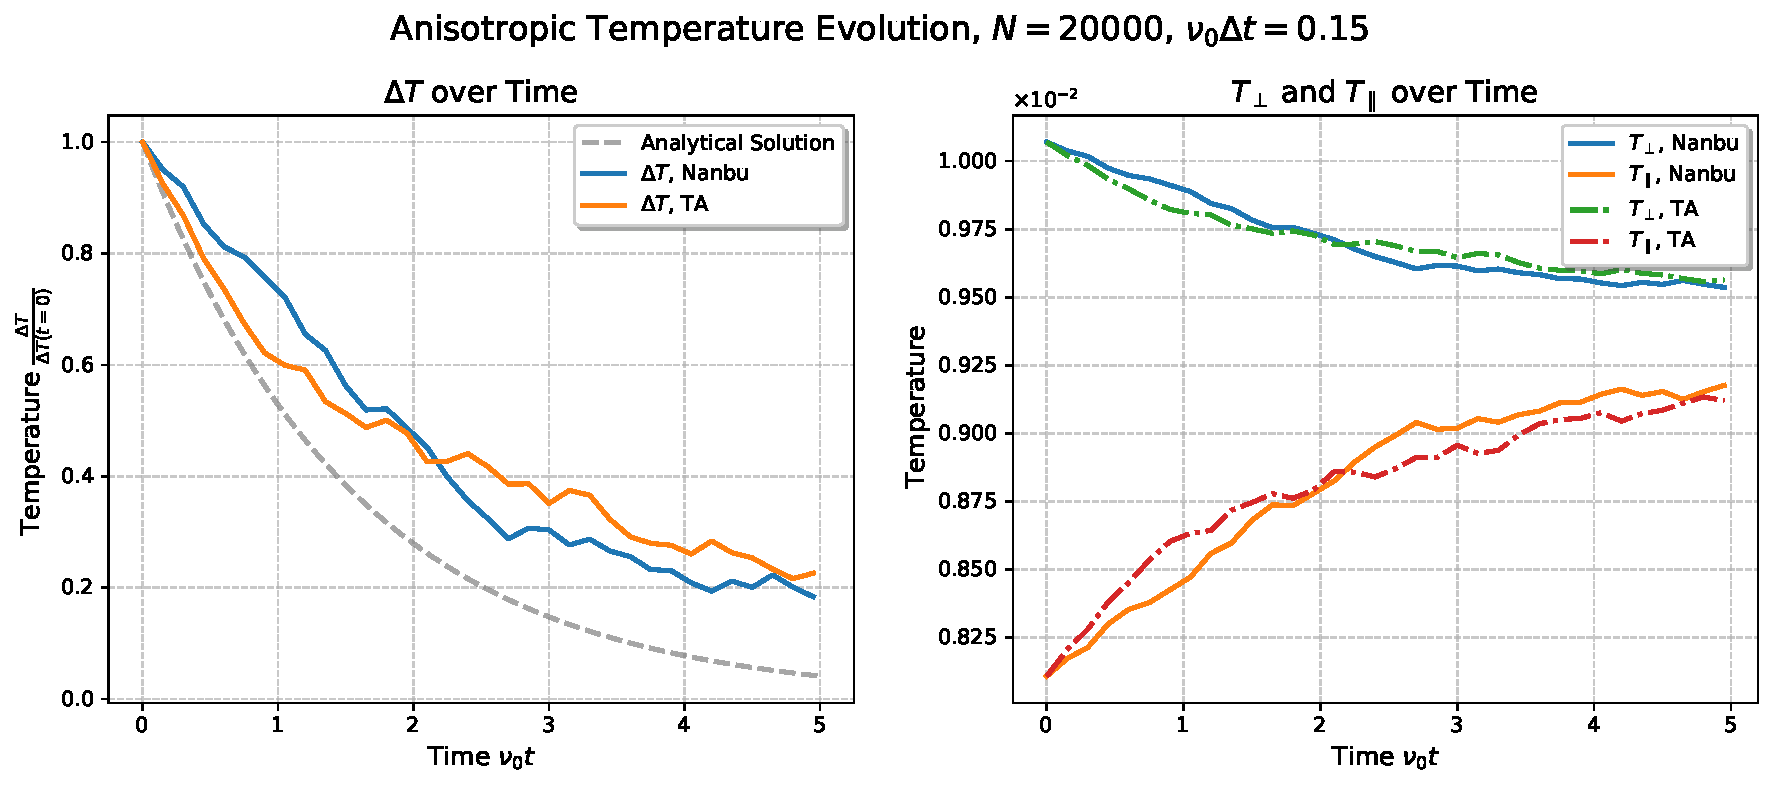
\includegraphics[width=\textwidth]{ressources/test1/anisotropic_T_example.pdf}
    \end{minipage}
    Gives the expected behaviour. 
    \begin{alertblock}{Problem}
        Line is slightly above the analytical solution!
    \end{alertblock}
\end{frame}

\begin{frame}{Accuracy Behaviour: Time vs. Step Sizes}
    \begin{minipage}{\textwidth}
        \centering
        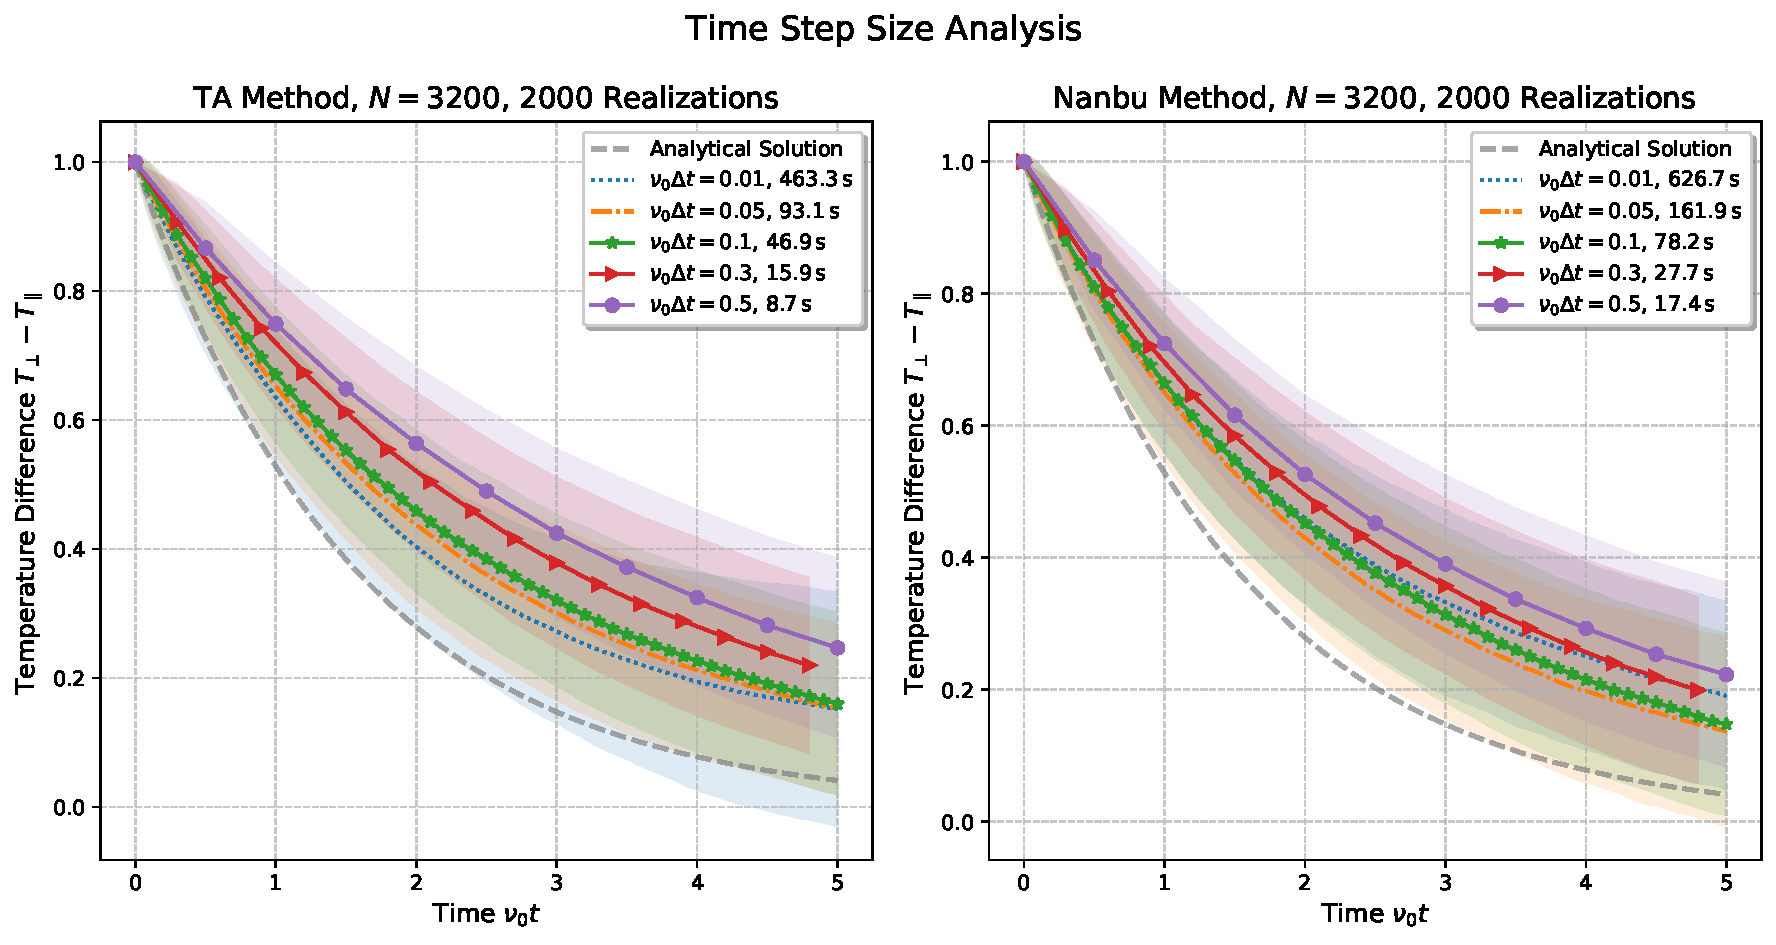
\includegraphics[width=\textwidth]{ressources/test1/temperature_diff_dT_combined_shaded.pdf}
    \end{minipage}
    Note: Converges with smaller time step sizes. \textsc{Nanbu} is \textit{very slightly} better for a given $\nu_0\Delta t$, but needs significantly longer.
\end{frame}

\begin{frame}{Precision Behaviour: Time vs. Step Sizes}
    \begin{minipage}{\textwidth}
        \centering
        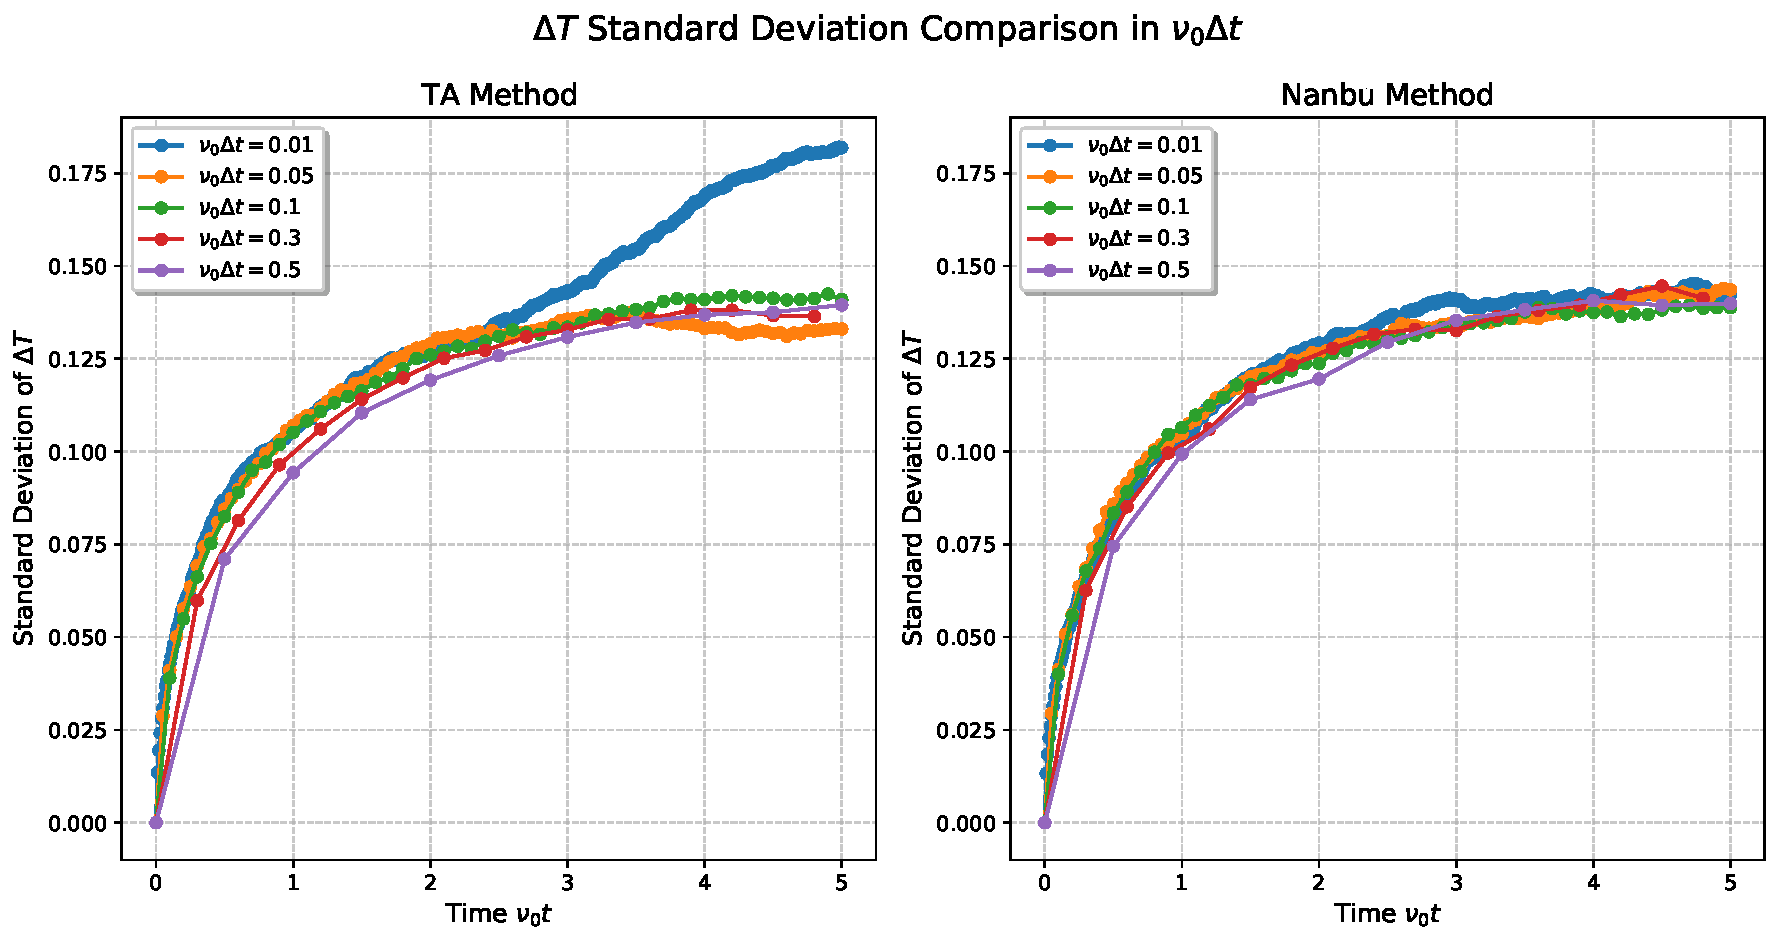
\includegraphics[width=\textwidth]{ressources/test1/temperature_std_dt_comparison.pdf}
    \end{minipage}
    Note: Standard deviation does not grow once the plasma is relaxed. Time step size has no influence. 
\end{frame}

\begin{frame}{Accuracy Behaviour: Time vs. Numbers of Particles}
    \begin{minipage}{\textwidth}
        \centering
        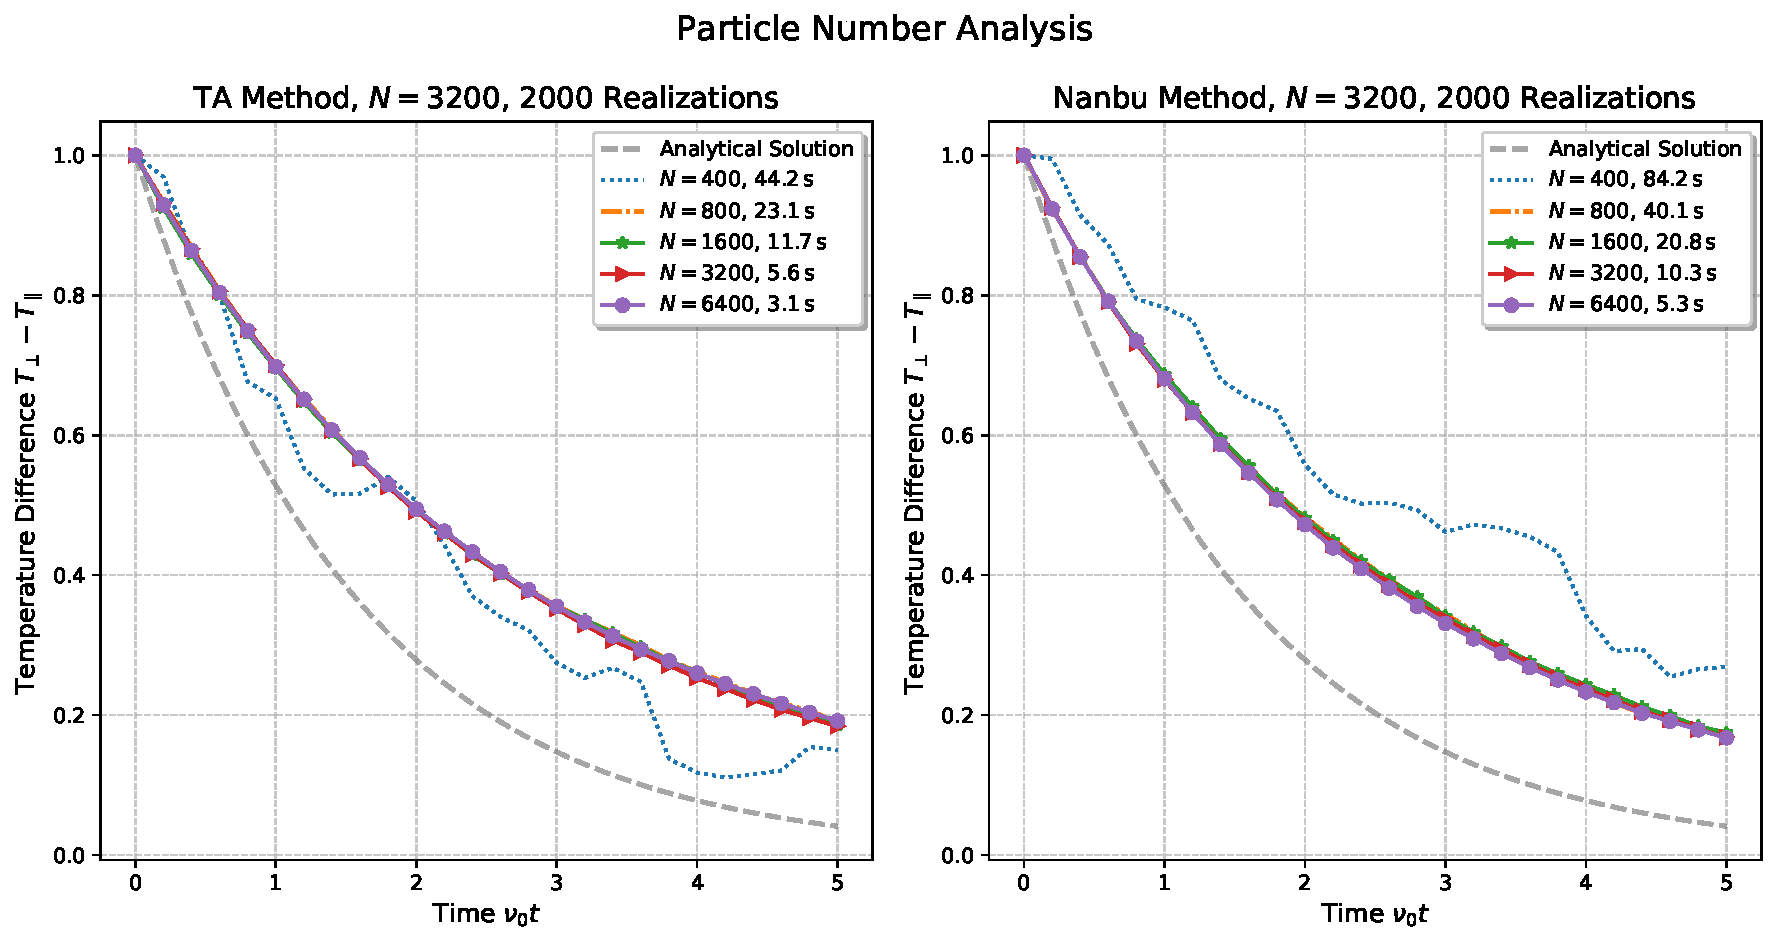
\includegraphics[width=\textwidth]{ressources/test1/temperature_diff_N_combined.pdf}
    \end{minipage}
    Note: Uses $\nu_0\Delta t=0.2$. Does not change accuracy, only affects precision (next two slide). 
\end{frame}

\begin{frame}{Precision Behaviour: Time vs. Numbers of Particles}
    \begin{minipage}{\textwidth}
        \centering
        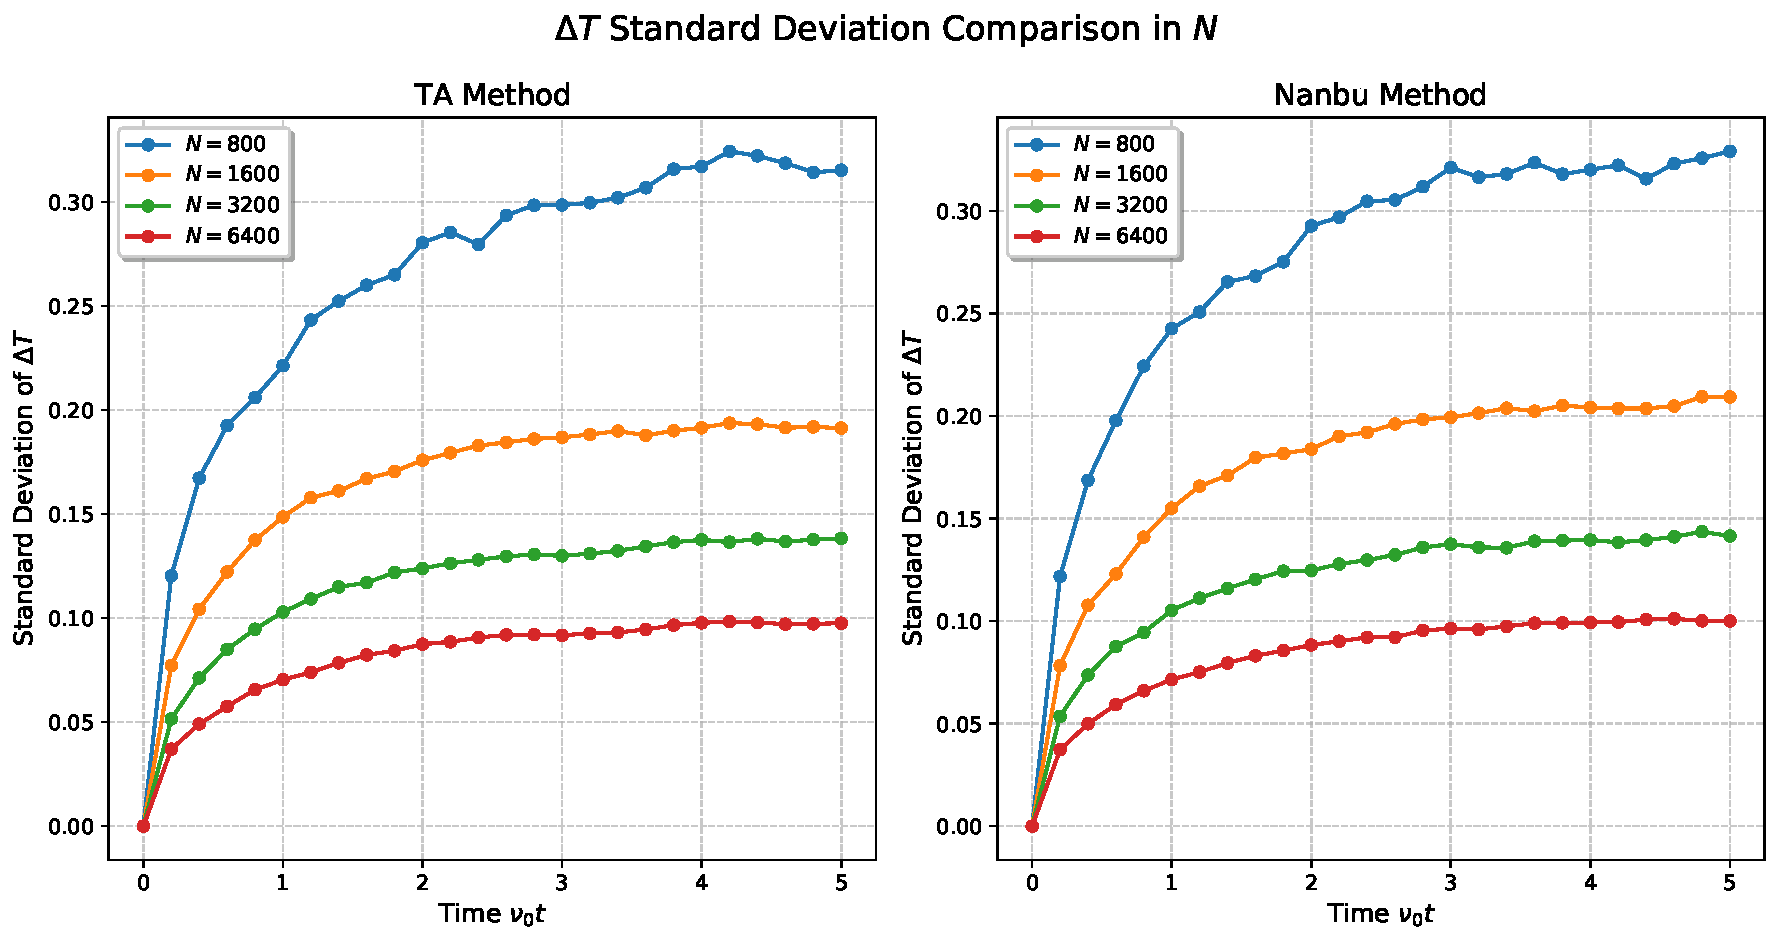
\includegraphics[width=\textwidth]{ressources/test1/temperature_std_N_comparison.pdf}
    \end{minipage}
    Note: Uses $\nu_0\Delta t=0.2$. More particles improve precision. \textsc{Nanbu} is \textit{very slightly} above TA.
\end{frame}







\subsection{\textsc{Dirac} Initial Distribution}

% Easy, when considering adaptive grid sizing!
\begin{frame}{\textsc{Dirac} Initial Distribution}
    Initial conditions:
    \begin{itemize}
        \item Initialize all velocities to $0$.
        \item Sample positions uniformly in a cube of length $d_x$ centered in the middle of the domain.
        \item Activate self-consistent electric field.
    \end{itemize}
    \vfill
    Example $d_x = 0.005 L$, 1000 particles, 500 timesteps and 10 realizations:
    \begin{minipage}{\textwidth}
        \centering
        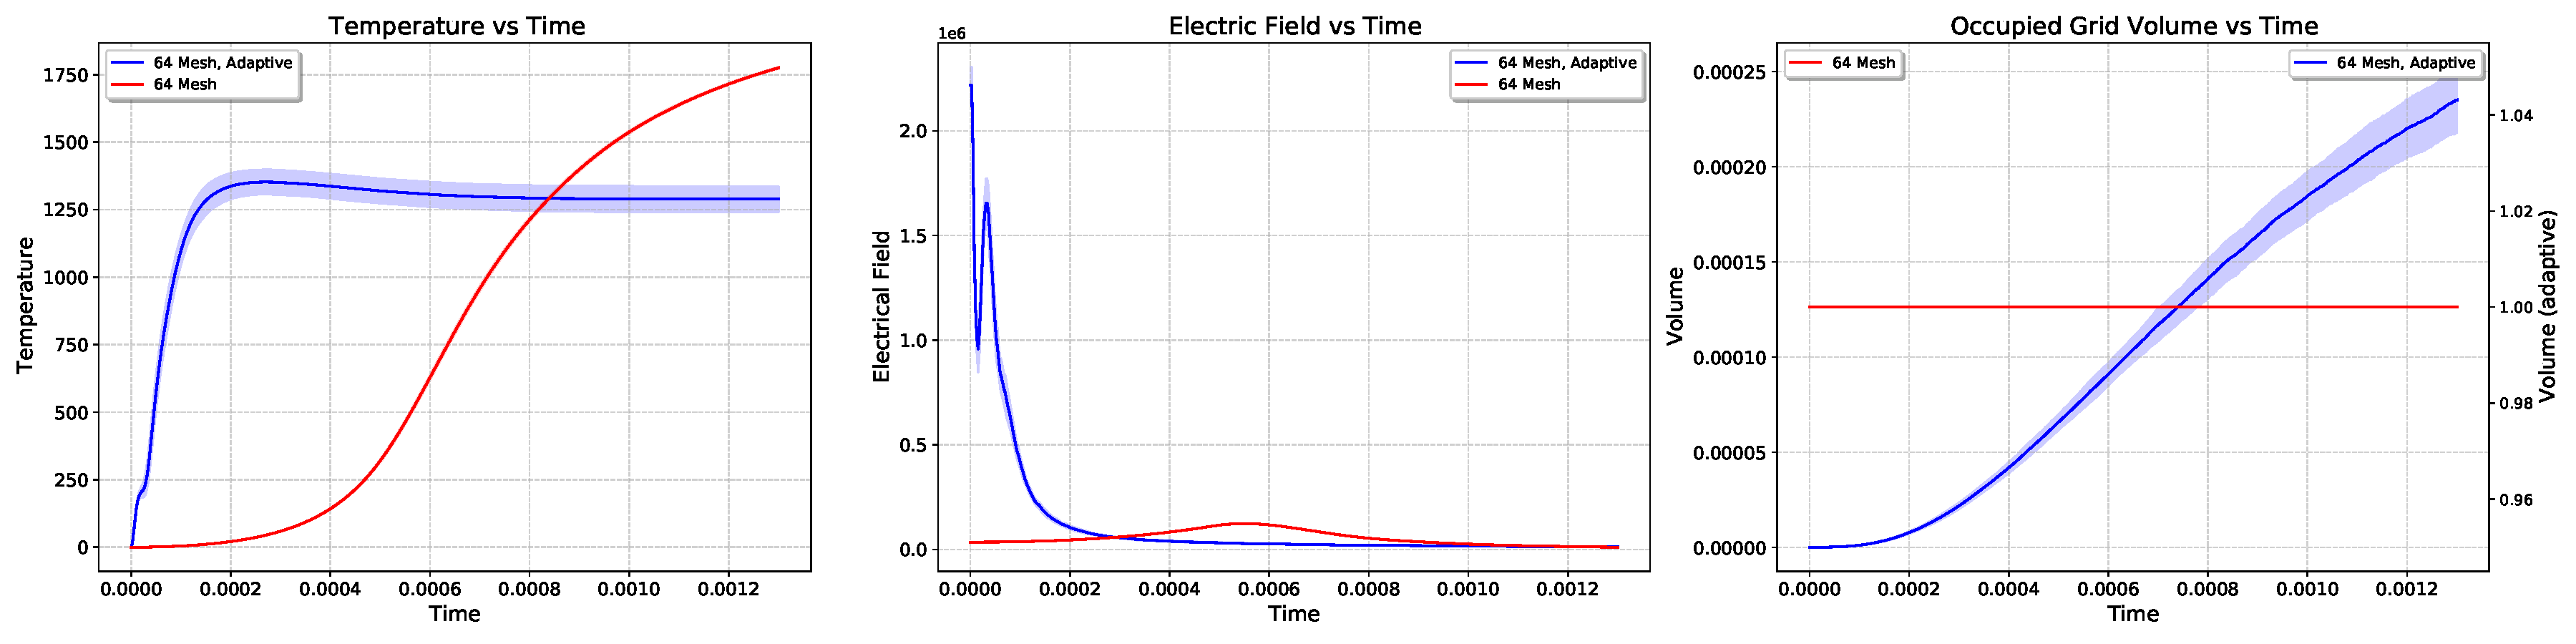
\includegraphics[width=\textwidth]{ressources/test2/T_E_V_comparison_adaptive_mesh_0.005.pdf}
    \end{minipage}
    Note: No adaptive grid means all particles are within one cell, delayed and damped initial ``surge'' of the electrical field. 
\end{frame}

\begin{frame}{Influence of Collisions}
    $d_x = 0.001$, $N = 1000$, $64$ adaptive grid, $500$ timesteps, $10$ realizations:
    \begin{minipage}{\textwidth}
        \centering
        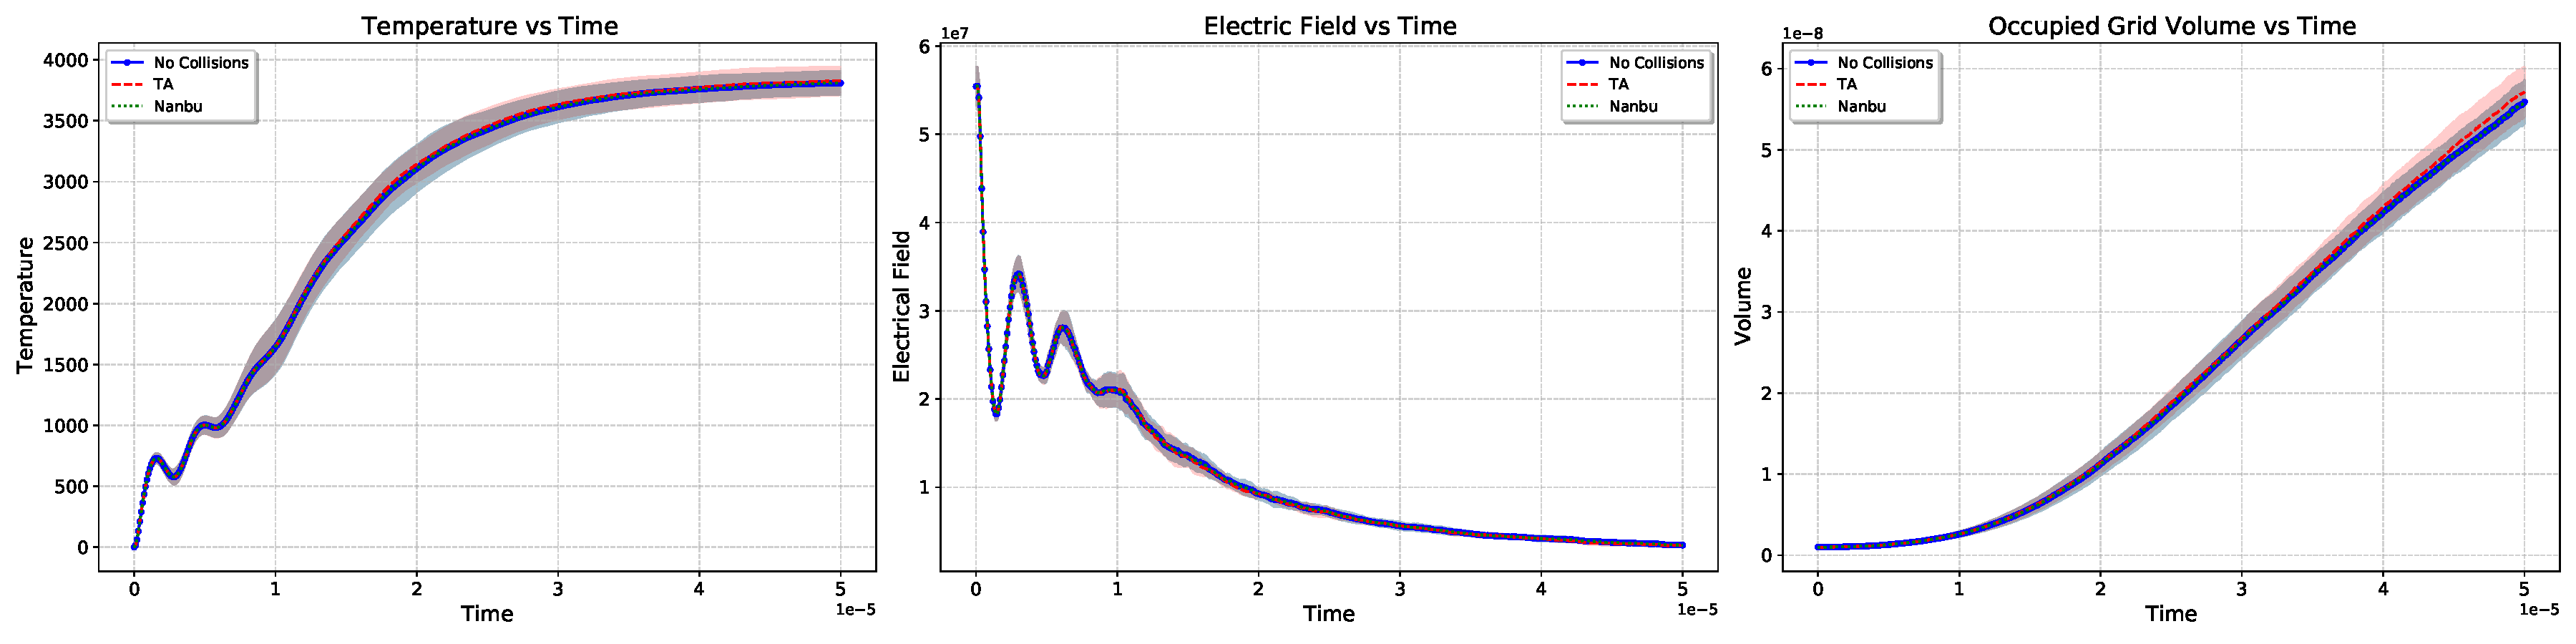
\includegraphics[width=\textwidth]{ressources/test2/T_E_V_comparison_collision_algos_0.00005.pdf}
    \end{minipage}
    \vfill
    Using $d_x = 0.95$ instead:
    \begin{minipage}{\textwidth}
        \centering
        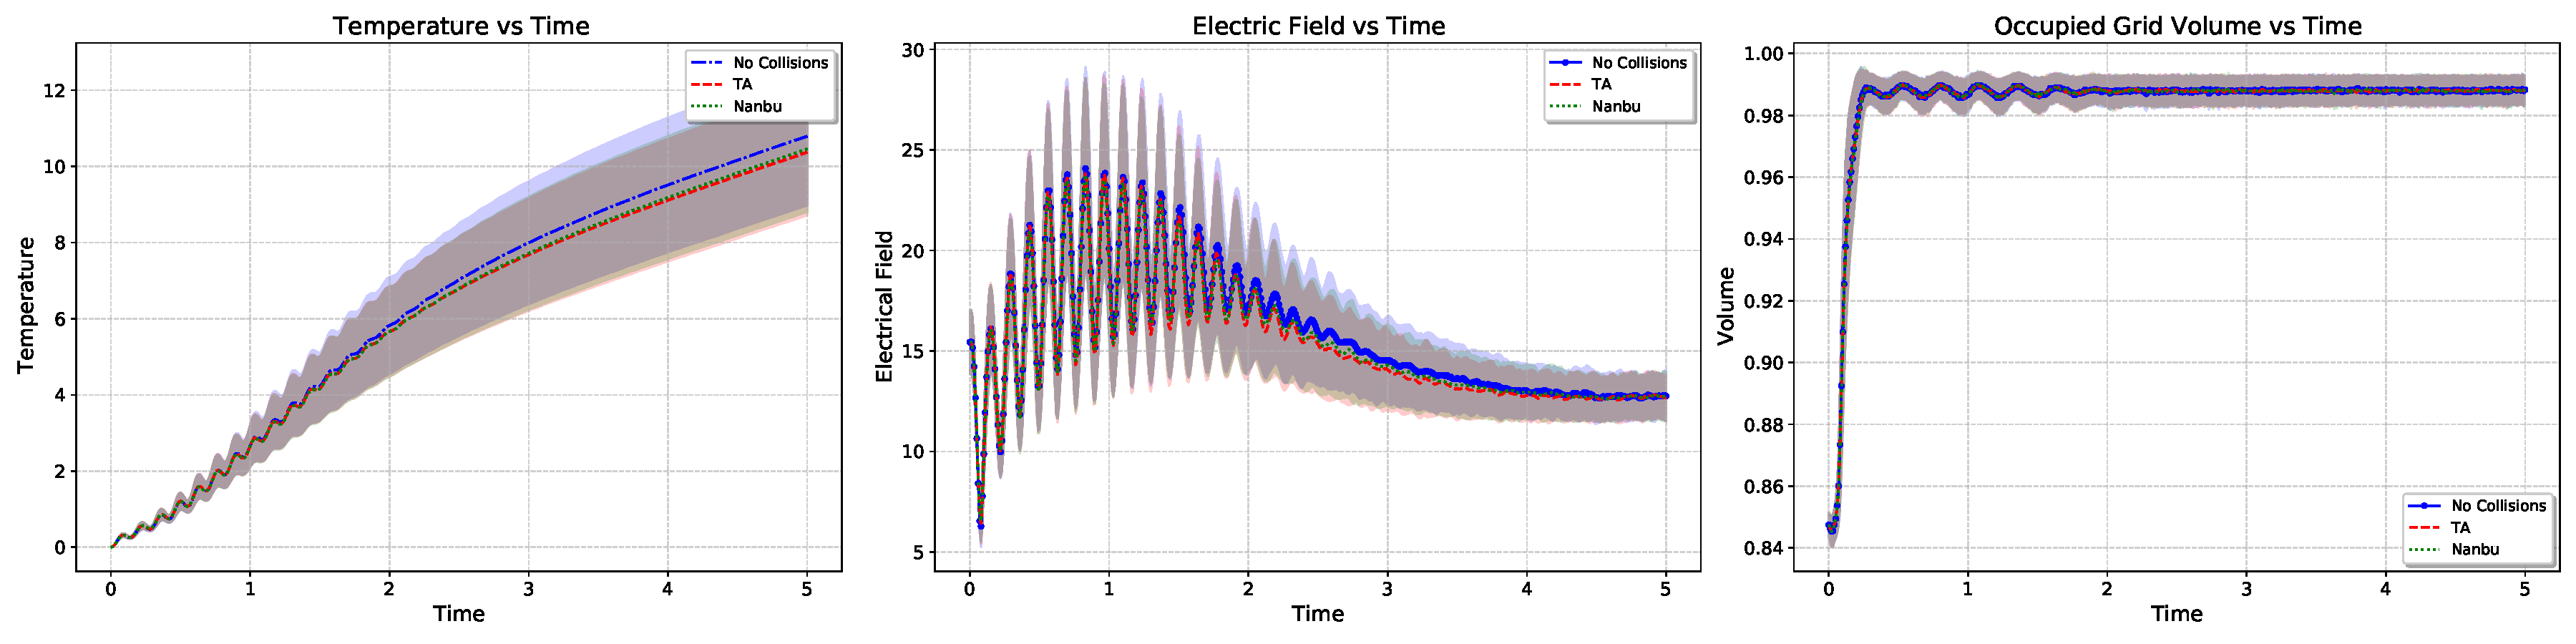
\includegraphics[width=\textwidth]{ressources/test2/T_E_V_comparison_collision_algos_5.0.pdf}
    \end{minipage}
    Note: Collisions important close to equlibrium/at big timesteps. Drastic change in $|\Delta\mathbf{v}|$ over time: small window where collisions matter. 
\end{frame}

\begin{frame}{Influence of Mesh Grid Size}
    Using $d_x = 0.01$, $N = 500$, $400$ timesteps over $10$ realizations with the adaptive grid:
    \begin{minipage}{\textwidth}
        \centering
        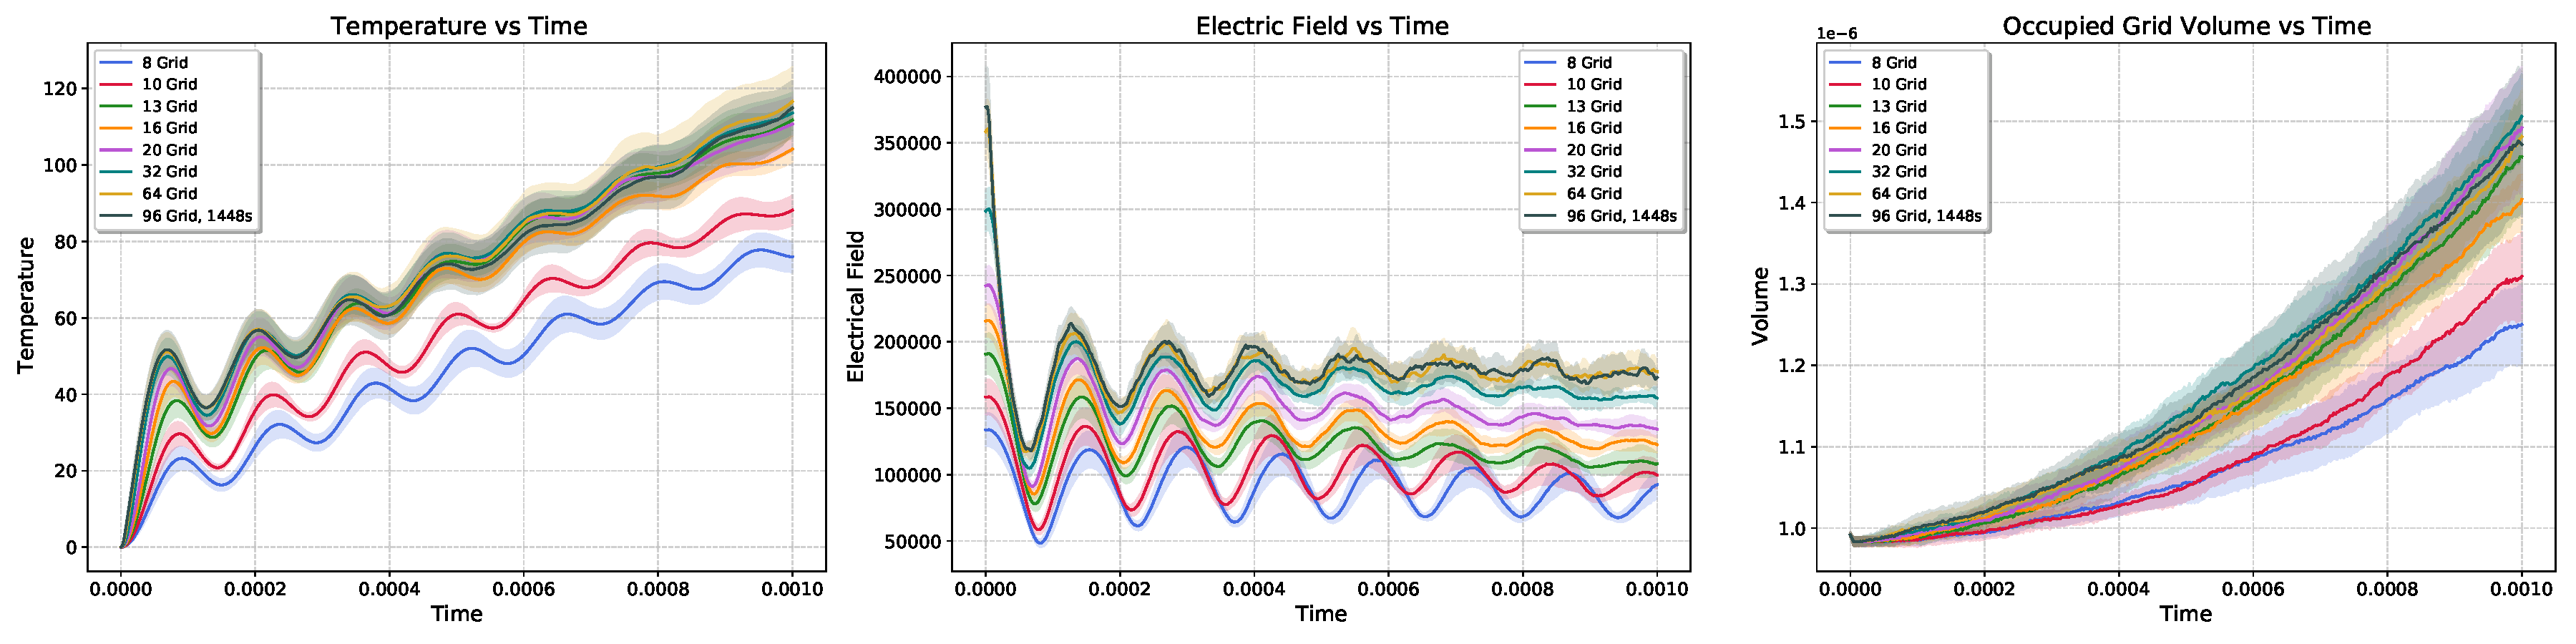
\includegraphics[width=\textwidth]{ressources/test2/T_E_V_comparison_grid_sizing.pdf}
    \end{minipage}
    Note: 
    \begin{itemize}
        \item Diminishing return within standard deviation after grid size $16$ (since the potential is almost uniform). 
        \item Field increases slightly with mesh size (faster space expansion and temperature increase). 
        \item Slight upwards trend in temperature: potential energy is converted to kinetic energy. 
    \end{itemize}
\end{frame}

\begin{frame}{Influence of (Time) Step Size}
    $d_x = 0.01$, $N = 500$, $16$ grid size over $100$ realizations and relative error:
    \begin{minipage}{\textwidth}
        \centering
        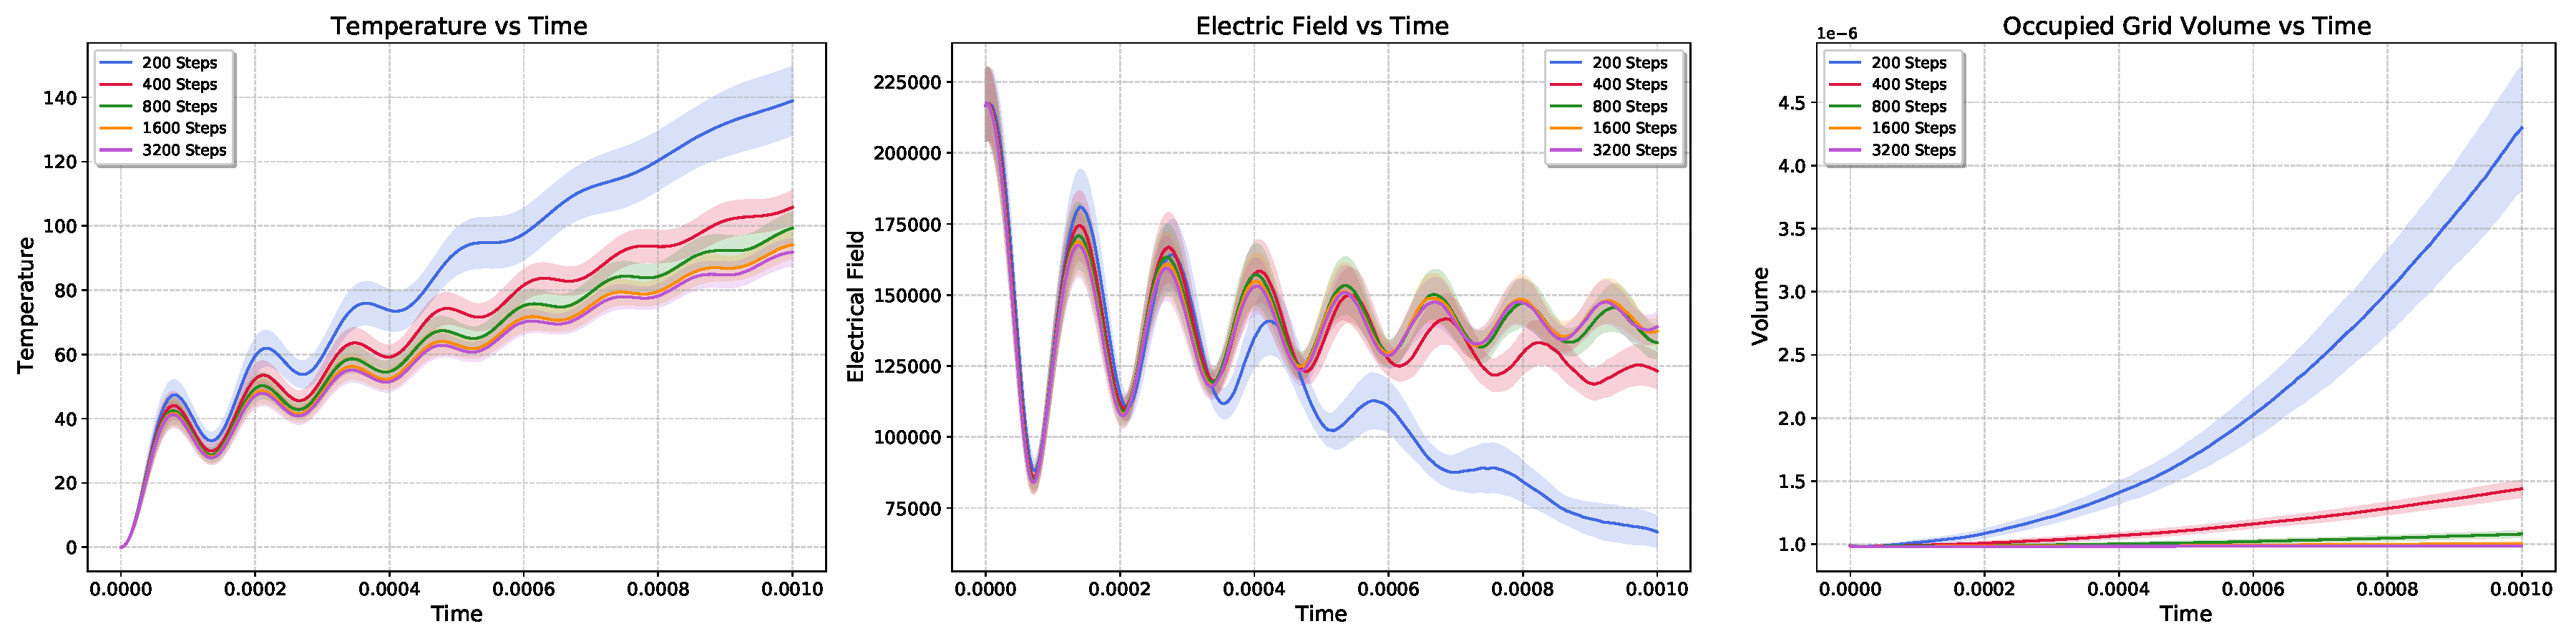
\includegraphics[width=\textwidth]{ressources/test2/T_E_V_comparison_timestepsize.pdf}
    \end{minipage}
    \begin{minipage}{\textwidth}
        \centering
        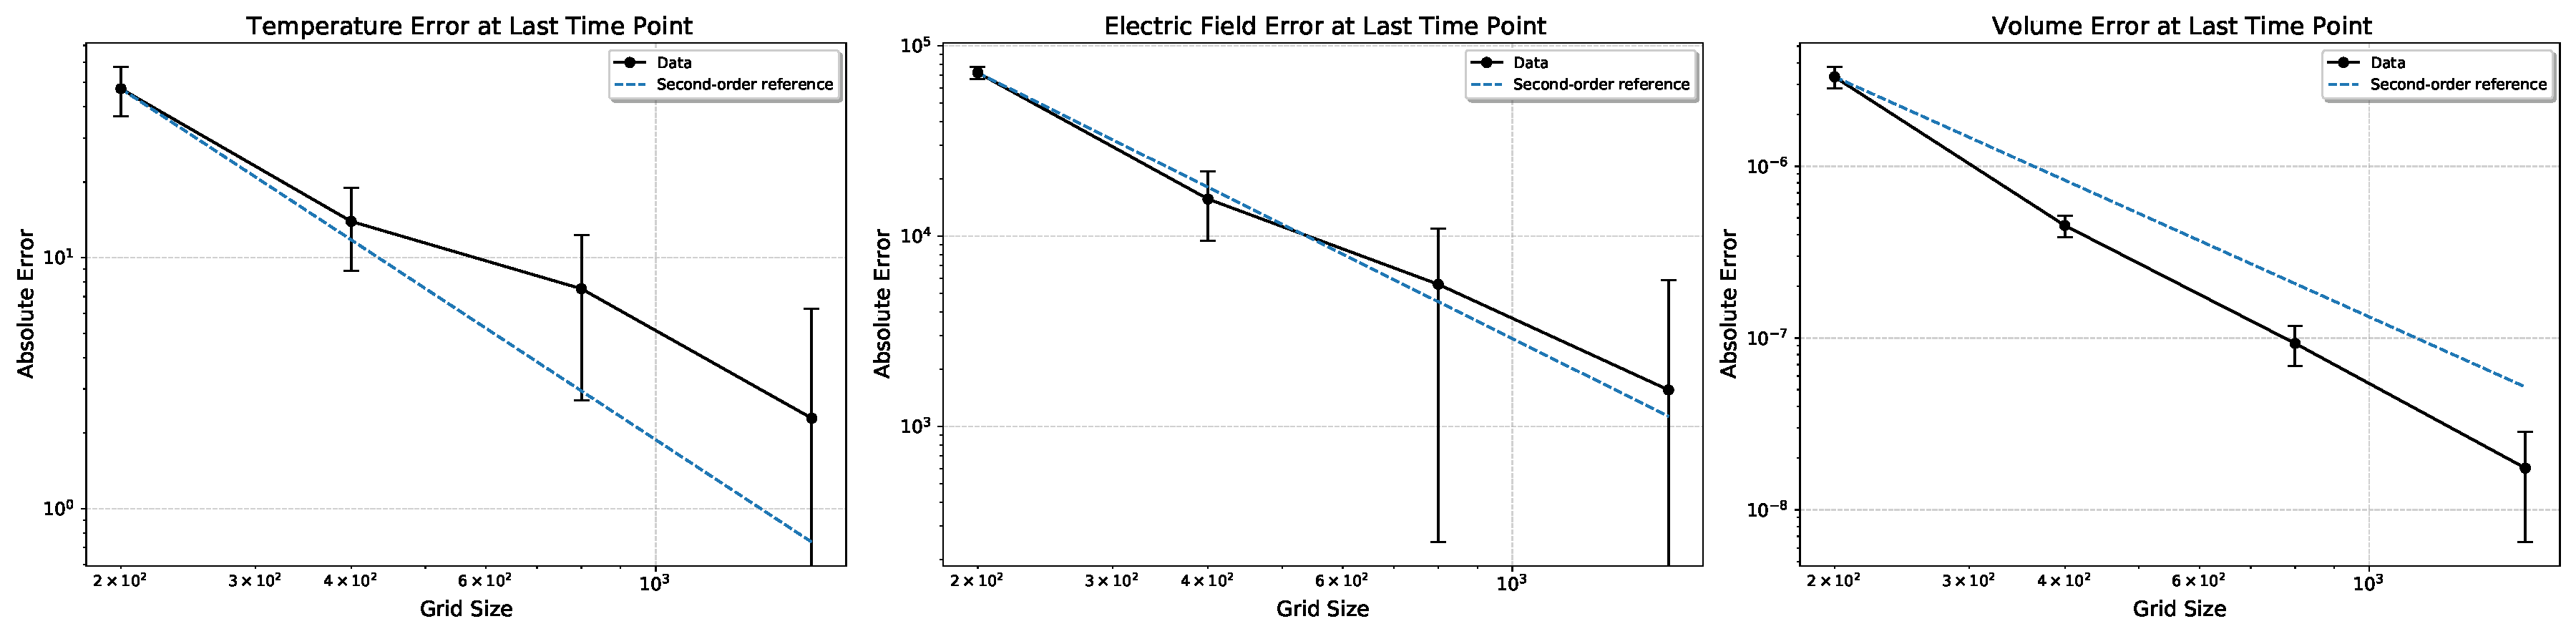
\includegraphics[width=\textwidth]{ressources/test2/T_E_V_comparison_timestepsize_errors.pdf}
    \end{minipage}
    Note: Roughly second order convergence, which is expected from a Leap-frog step.
\end{frame}


\subsection{Disorder Induced Heating of a Cold Sphere}

\begin{frame}{Disorder Induced Heating of a Cold Sphere}
    Initial conditions according to \cite[595]{Mitchell2015}:
    \begin{itemize}
        \item $L = 100\,\si{\micro\metre}$, $N=156055$, $n_0 = 6.67\cdot 10^{18}\,\si{\per\metre\cubed}$.
        \item Positions uniformly in sphere of radius $R = 17.74\,\si{\micro\metre}$.
        \item Velocities initially at $0$.
        \item Linear focusing force: apply equal and opposite radial electrical force (not accumulative, so fast particles will escape after some steps). 
        \item Additionally: reflect particles on the sphere ``shell''.
        \item Analyze the $x$-emmitance:
        $$
        \varepsilon_{x, \mathrm{rms}} = \sqrt{\langle x^2 \rangle \langle v^2 \rangle - (xv)^2}.
        $$
        \item Expect oscillation period of $\tau = 4.3 \cdot 10^{-11}\,\si{\second}$ and a final $x$-emittance value of $\varepsilon_{x,n}^\mathrm{eq} = 0.491 \,\si{\nano\metre}$.    
    \end{itemize}
\end{frame}

\begin{frame}{Mesh-Grid Size Comparison}
    $x$ emmitance (left) for different (adaptive) grid sizes and 1 realization:
    \begin{minipage}{\textwidth}
        \centering
        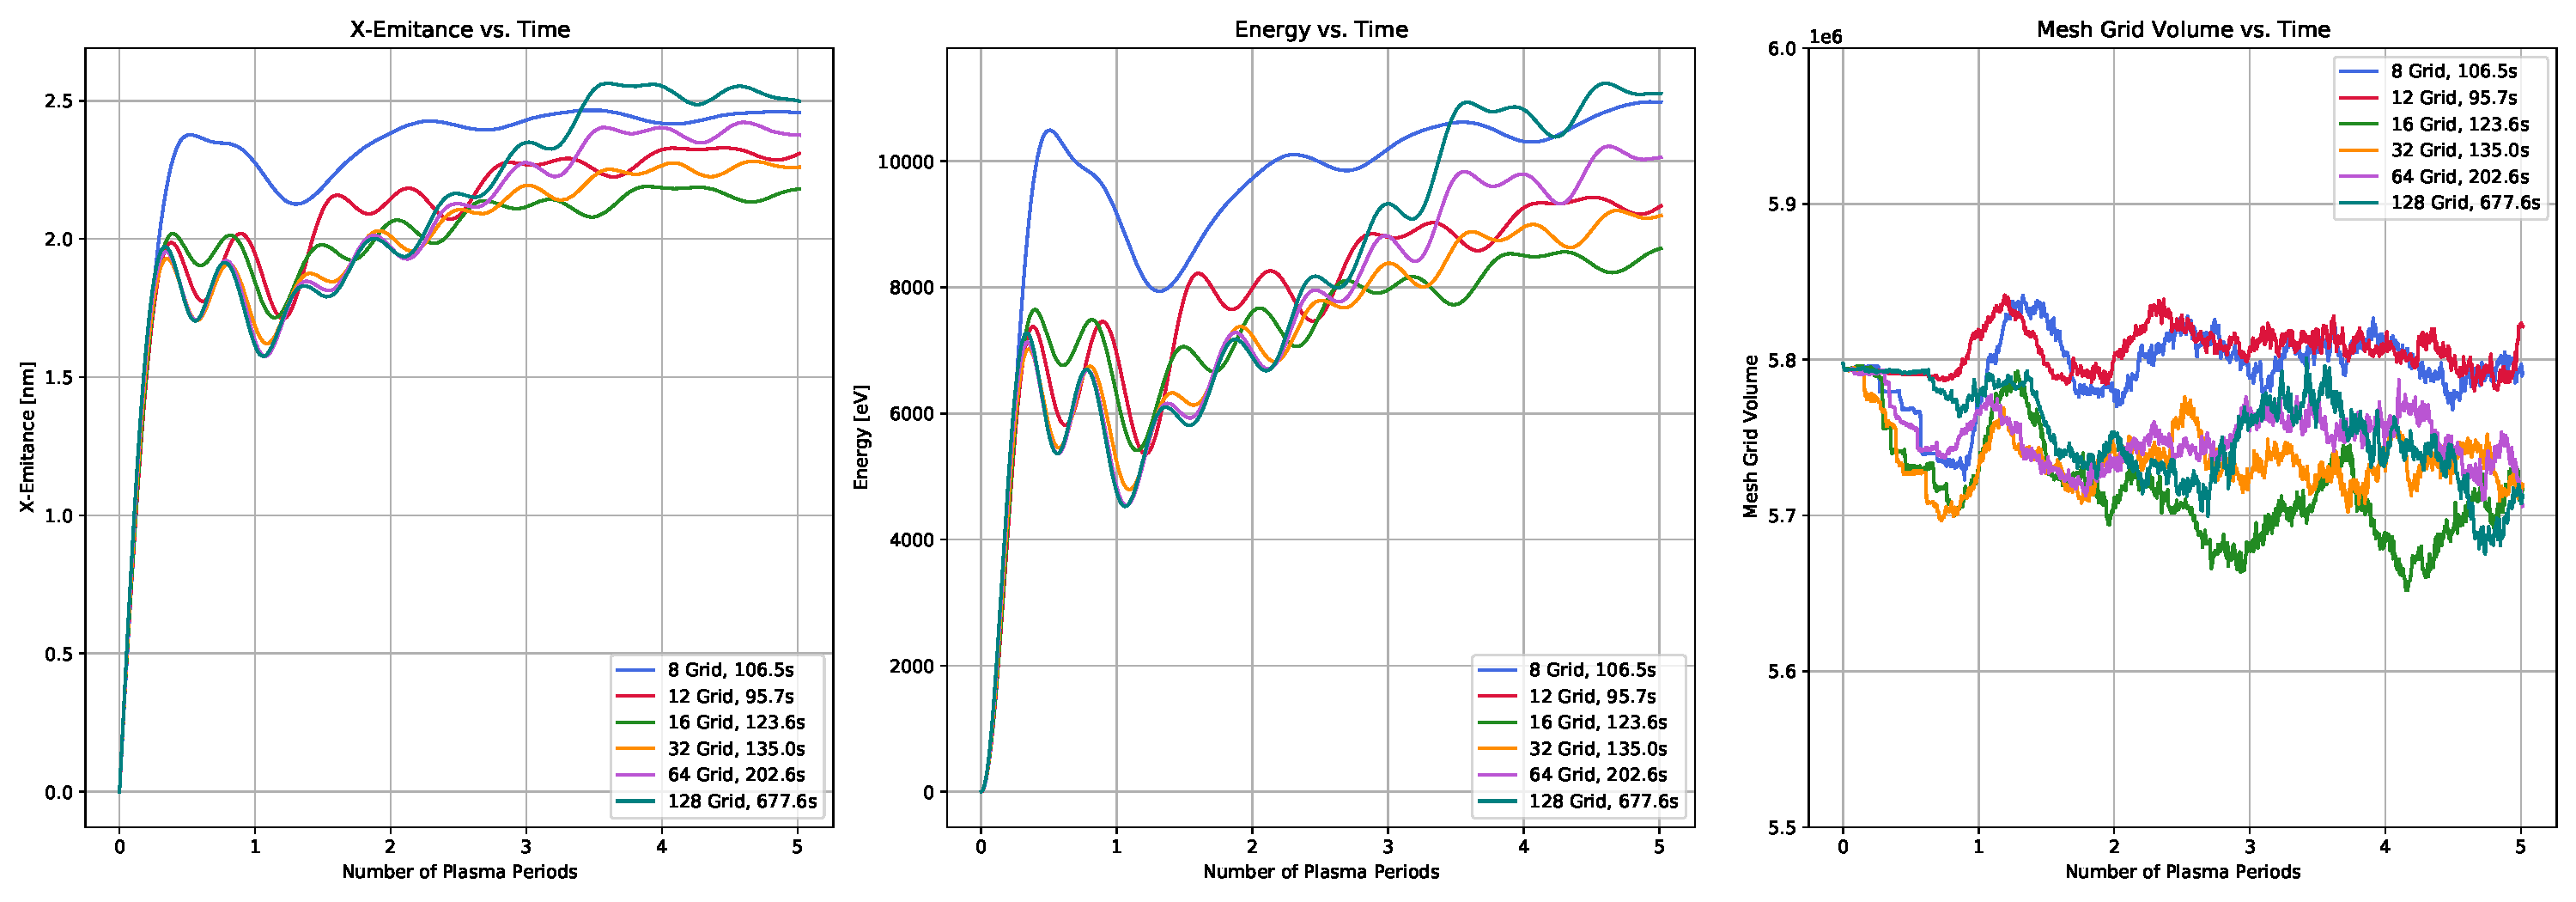
\includegraphics[width=\textwidth]{ressources/test3/cold_sphere_grid_comparison.pdf}
    \end{minipage}
    \begin{itemize}
        \item The confinement works well (right plot).
        \item Dominant frequencies from FFT on the 64 grid emittance:
        $$
        2.16\cdot 10^{-11}\,\si{\second},
        \qquad 6.49\cdot 10^{-11}\,\si{\second},
        \qquad 3.24\cdot 10^{-11}\,\si{\second} .
        $$
        \item Diminishing returns at small grids due to homogeneity of particles.
        \item Missing ``smoothness'' correlates with spikes in mesh grid volume. % (scaling or precision issue?)
    \end{itemize}
\end{frame}

\begin{frame}{Collision Algorithm Comparison}
    Using different collision algorithms and $5$ realizations each:
    \begin{minipage}{\textwidth}
        \centering
        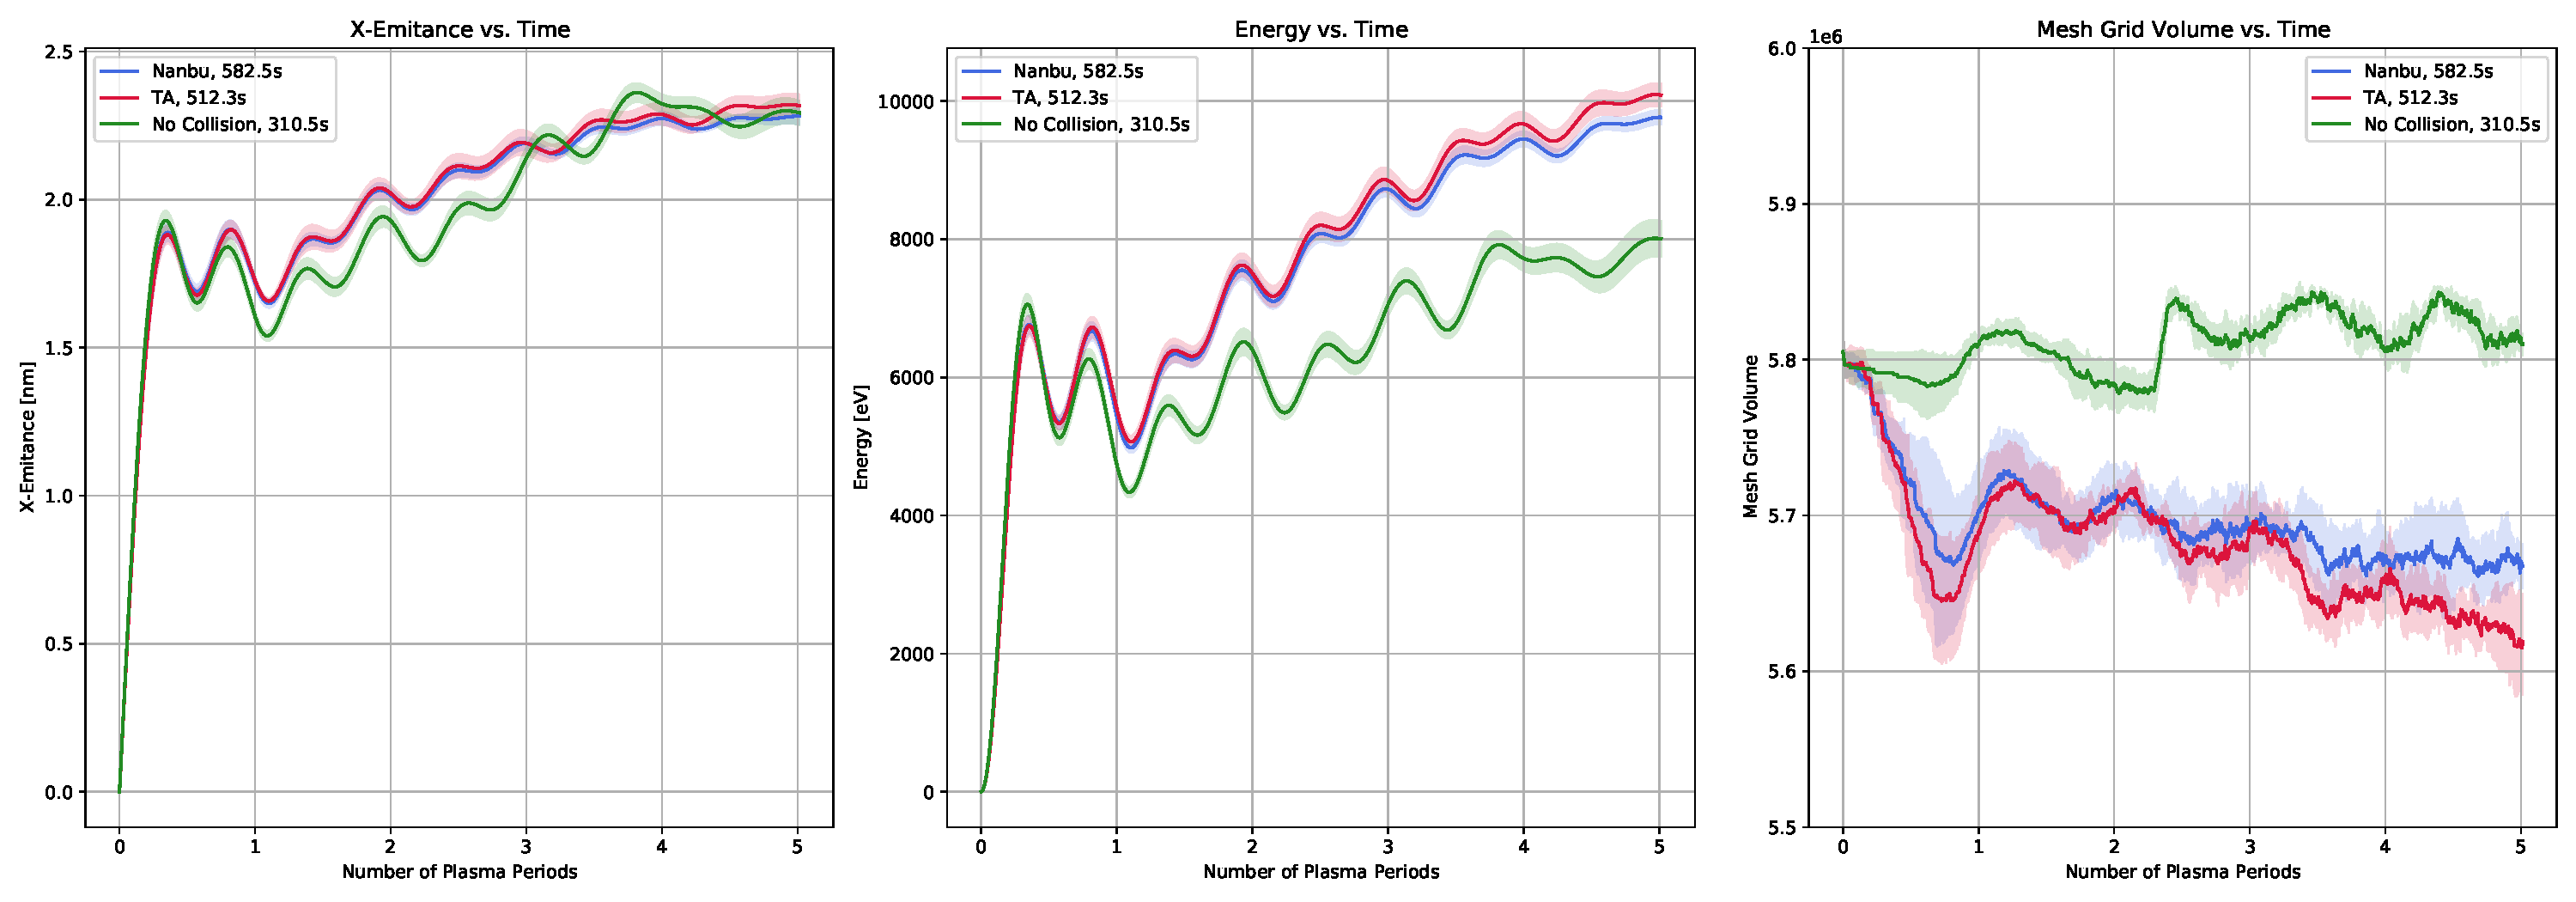
\includegraphics[width=\textwidth]{ressources/test3/cold_sphere_collision_algo_comparison.pdf}
    \end{minipage}
    \begin{itemize}
        \item As in \cite[595]{Mitchell2015}: no collisions mean lower emittance.
        \item Collisions significant shortly in the beginning (as before).
        \item No significant difference between TA and \textsc{Nanbu}.
        \item Overshoots expected emittance value (as before).
    \end{itemize}
\end{frame}


\section{Problems and Comparison Differences}

\subsection{Deviation from \cite{Wang2008} for \textsc{Trubnikov}'s Test}

\begin{frame}{Trubnikov ``Reference'' Solution: Test Run}
    \begin{minipage}{\textwidth}
        \centering
        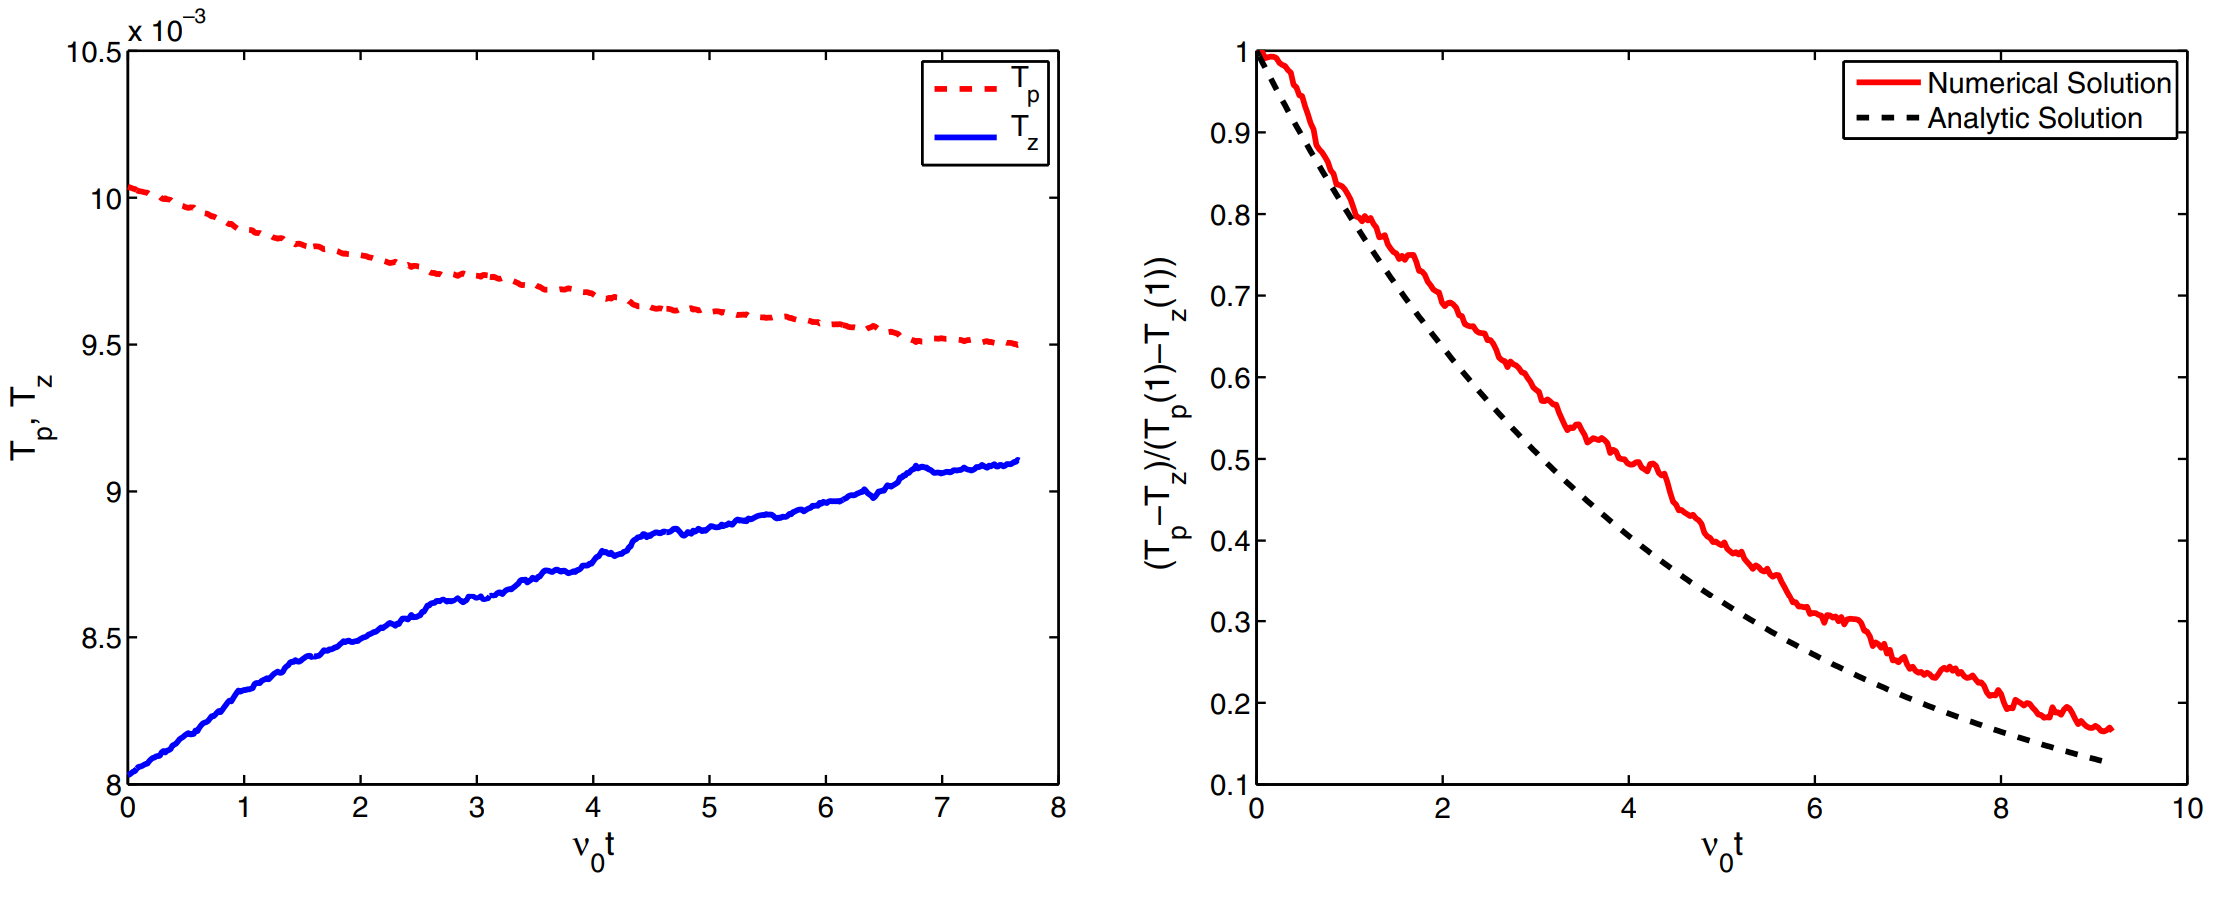
\includegraphics[width=\textwidth]{ressources/test1/Wang_anisotropic.png}
    \end{minipage}
    Note: similar behaviour, but simulation slightly above analytical solution.
\end{frame}

\begin{frame}{Trubnikov ``Reference'' Solution: Time Step Size}
    \begin{minipage}{\textwidth}
        \centering
        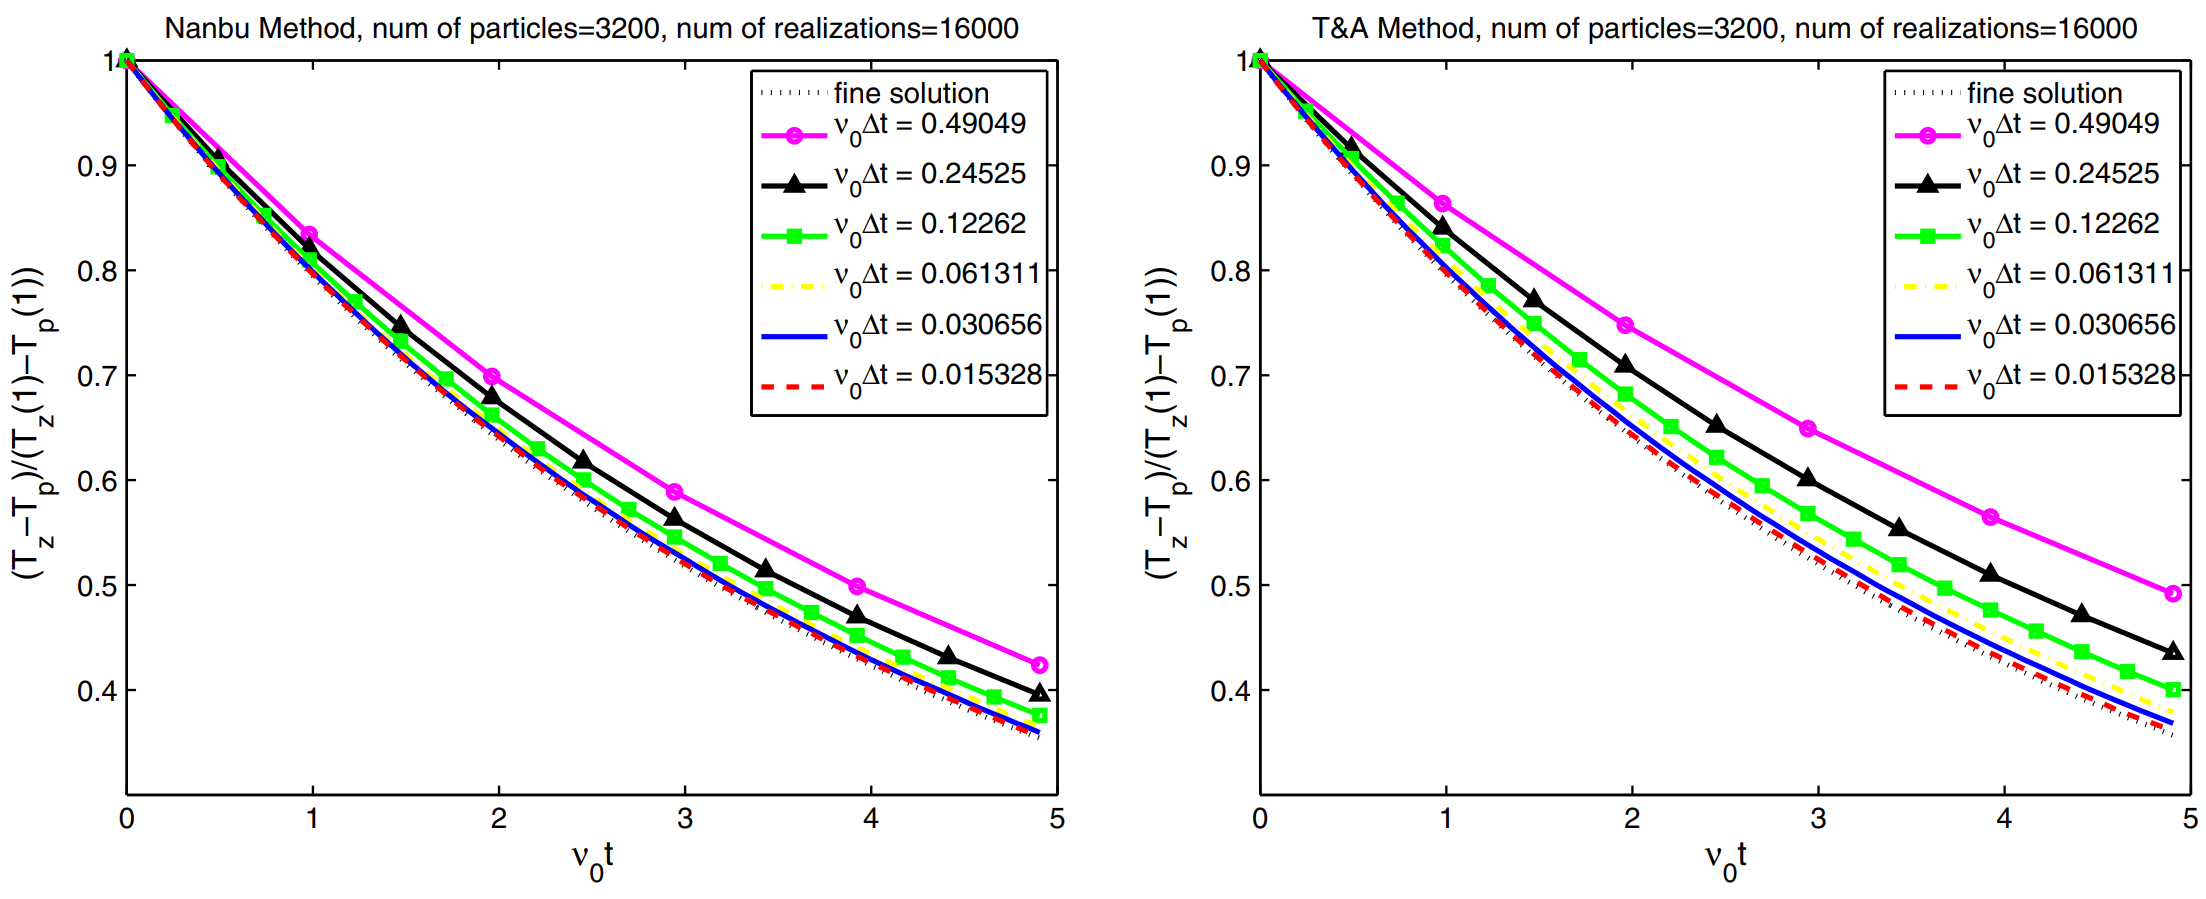
\includegraphics[width=\textwidth]{ressources/test1/Wang_dT.png}
    \end{minipage}
    \begin{itemize}
        \item \cite{Wang2008} does not use the analytical solution $\rightarrow$ same convergence discrepancy.
        \item No explanation: uses a fine solution without providing any details. 
        \item \textsc{Nanbu} has slightly better accuracy (does not mention computation time).
    \end{itemize}
\end{frame}

\begin{frame}{Trubnikov ``Reference'' Solution: Number of Particles}
    \begin{minipage}{\textwidth}
        \centering
        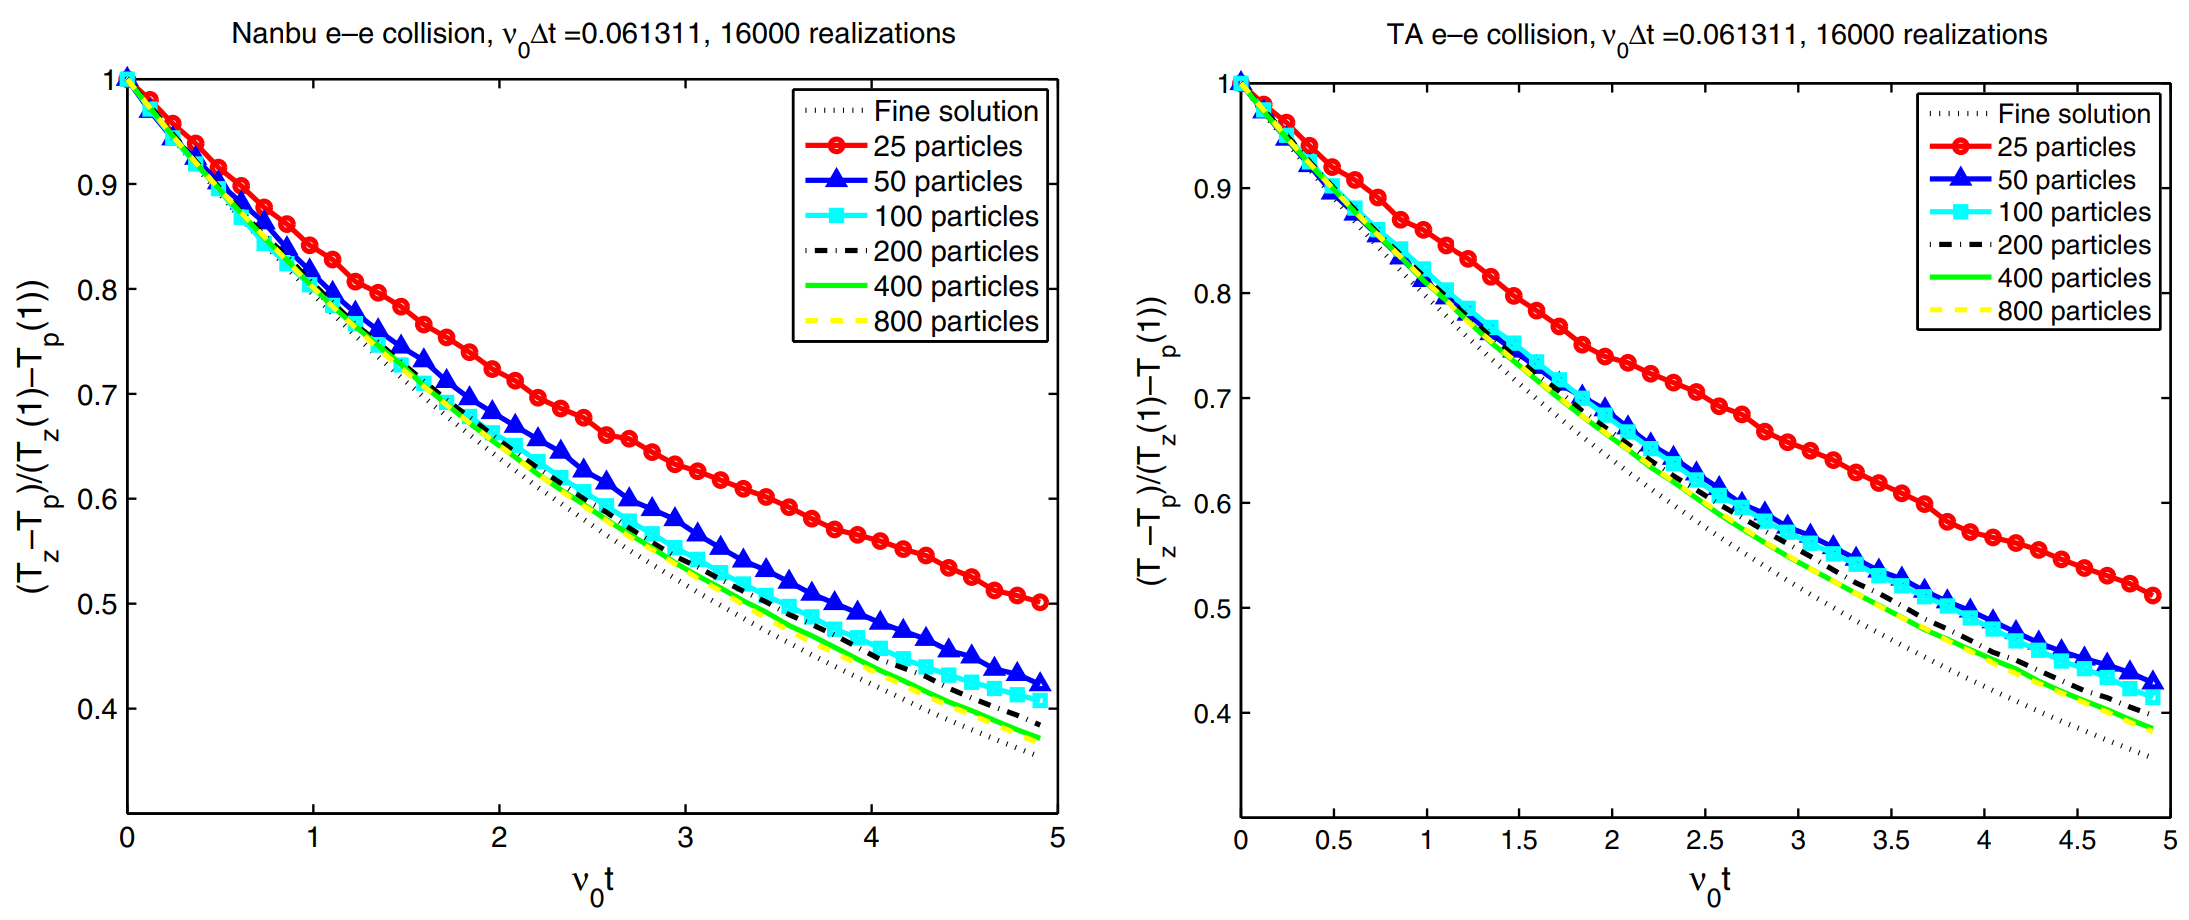
\includegraphics[width=\textwidth]{ressources/test1/Wang_N.png}
    \end{minipage}
    \begin{itemize}
        \item Paper notes convergence in $N$.
        \item Does not mention the analytical solution and uses a fine solution.
        \item Looking at the first graph, their analytical solution is also significantly lower.
        \item \cite{Wang2008} never mentioned their domain size, $n$ or $\ln\Lambda$, $\lambda_\mathrm{D}$ calculation.
    \end{itemize}
\end{frame}


\subsection{Cold Sphere $\gg$ \textsc{Debye}-Length}

\begin{frame}{Insignificance of Collisions During Cold Sphere Heating}
    The program has to options:
    \begin{itemize}
        \item Calculate $\lambda_\mathrm{D}$, compute collisions in a grid of size $\frac{L}{\lambda_\mathrm{D}}$.
        \item Compute collisions per usual grid cell.
    \end{itemize}
    Problem ($k_\mathrm{B}T_\mathrm{eq} \approx 1.96\si{\milli\electronvolt}$):
    $$
    \lambda_\mathrm{D} = \sqrt{\frac{\varepsilon_0 k_\mathrm{B} T}{n q^2}} \approx 0.13\,\si{\micro\metre} .
    $$
    \begin{itemize}
        \item Gives on average $0.06$ particles per cell.
        \item Confirms marginal significance of collisions in this context.
    \end{itemize}
    Therefore: here obtained result makes sense!
\end{frame}


\subsection{Field Solver Scaling Issue}

% Depending the adaptive gridsize
\begin{frame}{Adaptive Grid Sizing: Scaling Problem}
    Same simulation, no adaptive grid and different grid sizes:
    \begin{minipage}{\textwidth}
        \centering
        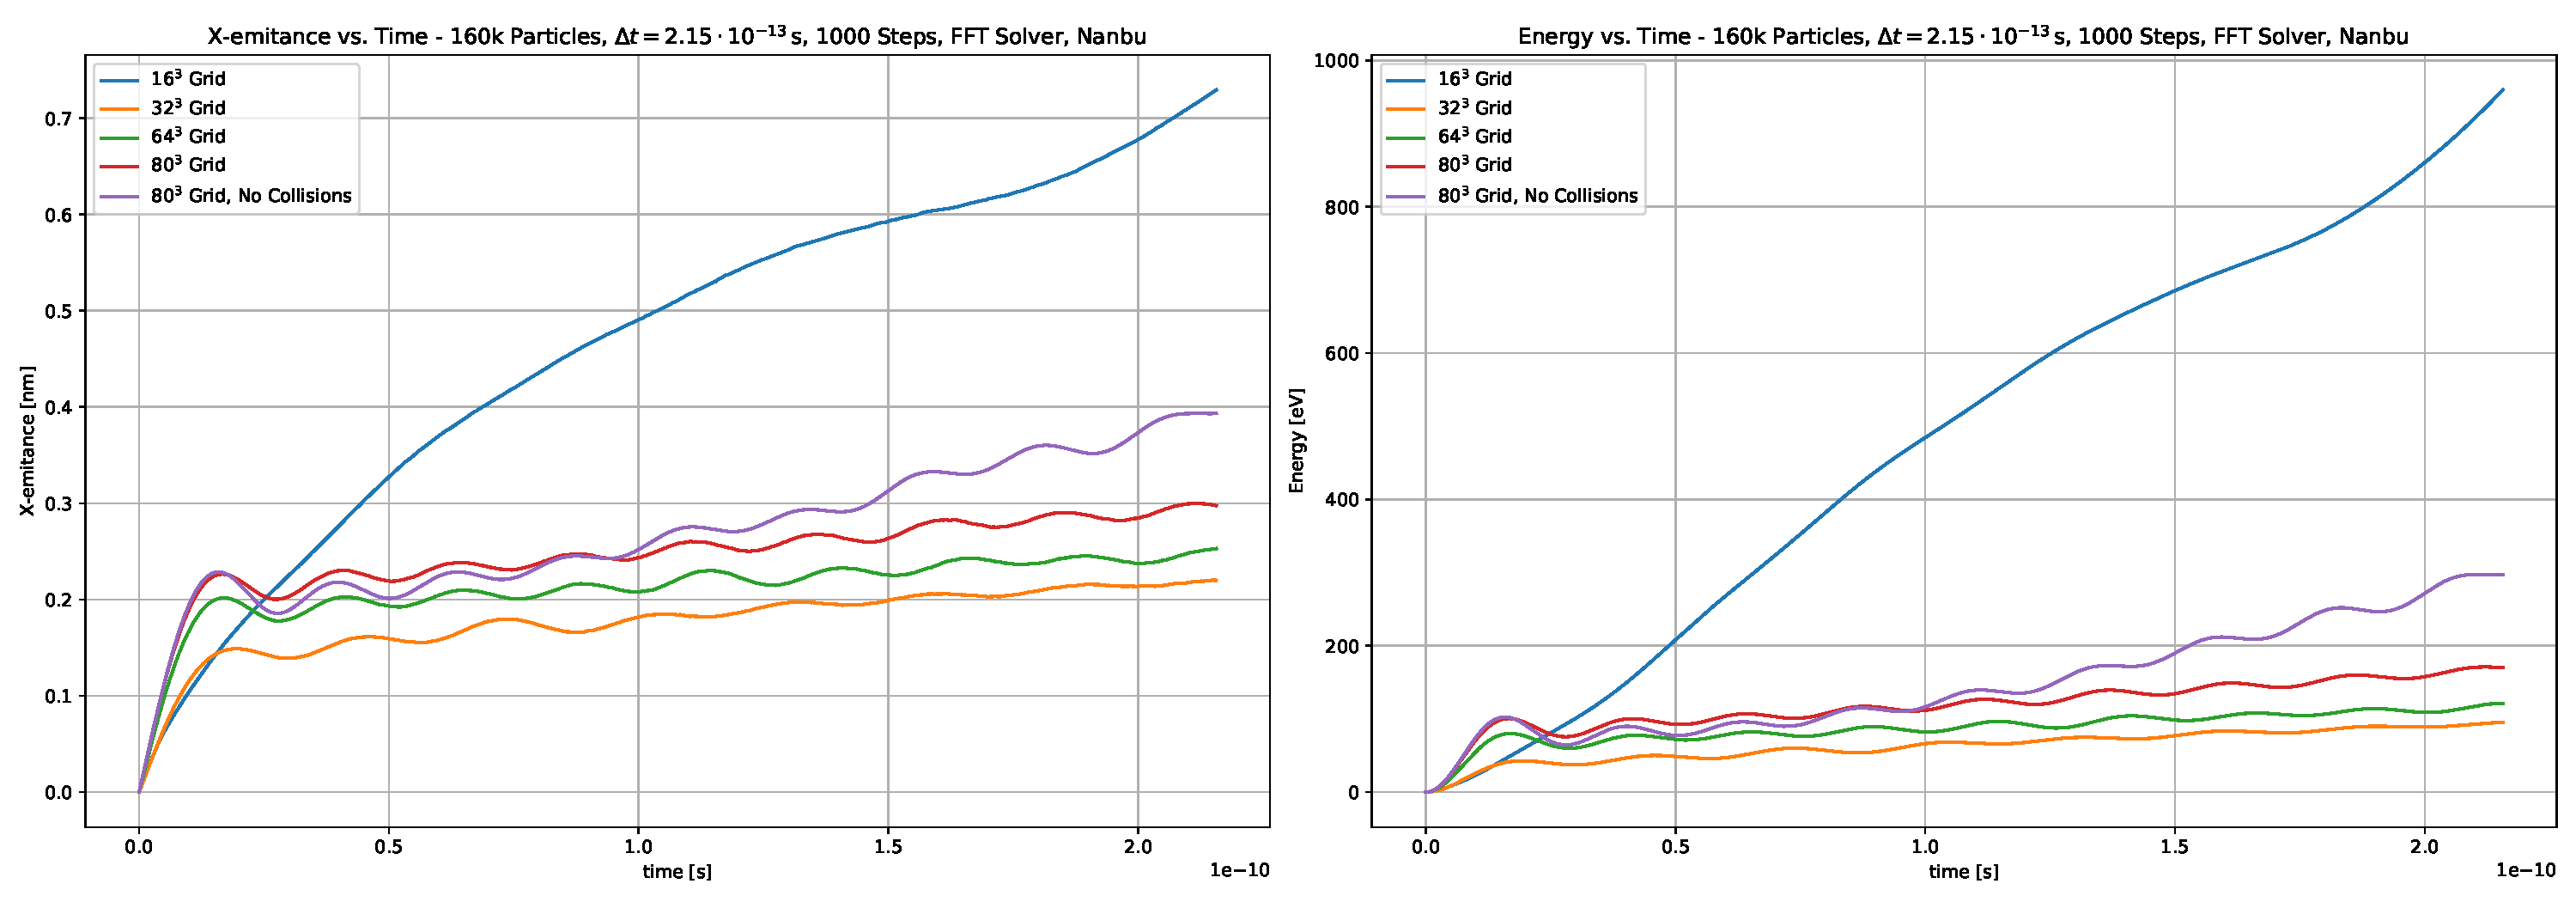
\includegraphics[width=\textwidth]{ressources/additional/disorder_heating_grid_comparison.pdf}
    \end{minipage}
    \begin{itemize}
        \item Oscillations are way more regular.
        \item Is way closer to the expected equilibrium ($0.491\,\si{\nano\metre}$).
        \item Oscillation period seems unchanged.
    \end{itemize}
\end{frame}

\begin{frame}[fragile]{Adaptive Grid Sizing: Implementation}
    \begin{itemize}
        \item Inside \verb|advance()|, calculate self-consistent field using:
    \end{itemize}
\begin{lstlisting}
if (this->computeSelfField_m) {
    if (this->adjust_field_dims) adjustFieldMeshDimensions(); 
    this->par2grid();
    this->fsolver_m->runSolver();
    this->grid2par();
    if (this->adjust_field_dims) resetBoundaries();
}
\end{lstlisting}
    \begin{itemize}
    \item Adjust grid dimensions, such that every particle is barely in it.
    \item After solving and interpolating onto the particles, the boundaries are resetted to the value before.
    \end{itemize}
\end{frame}


\begin{frame}[fragile]{Adaptive Grid Sizing: Adjust Dimensions}
\begin{lstlisting}
void adjustFieldMeshDimensions() {
    std::shared_ptr<ParticleContainer_t> pc = this->pcontainer_m;
    auto *mesh = &this->fcontainer_m->getMesh();
    auto *FL   = &this->fcontainer_m->getFL();

    // Calculate the maximum and minimum of all particle coordinates using Kokkos
    view_type* R               = &(pc->R.getView());
    MinMaxReducer<Dim> minMax;
    findMinMax(R, minMax); 
    Vector_t<double, Dim> maxR = minMax.max_val, minR = minMax.min_val;
    
    // Now figure out componentwise global min/max values
    Vector_t<double, Dim> globalMaxR, globalMinR;
    for (size_t i = 0; i < Dim; i++) {
        ippl::Comm->reduce(&maxR[i], &globalMaxR[i], 1, std::greater<double>());
        ippl::Comm->reduce(&minR[i], &globalMinR[i], 1, std::less<double>());
    }

    // Calculate new mesh spacing 
    Vector_t<double, Dim> hr = (globalMaxR-globalMinR) / mesh->getGridsize(); 
    
    // set the origin and mesh spacing of the mesh via
    mesh->setMeshSpacing(hr);
    mesh->setOrigin(globalMinR); 

    this->rmin_m = globalMinR;
    this->origin_m = globalMinR;
    this->rmax_m = globalMaxR;
    this->hr_m = hr;

    extLayoutUpdate(FL, mesh);
    pc->update();
}
\end{lstlisting}
    \begin{itemize}
        \item Manually reset \verb|rmin|, \verb|rmax| and recalculate \verb|hr|.
        \item Update the mesh container.
    \end{itemize}
\end{frame}


\begin{frame}[fragile]{Adaptive Grid Sizing: Extended Layout Update}
\begin{lstlisting}
void extLayoutUpdate(ippl::FieldLayout<Dim>* fl, ippl::UniformCartesian<T, Dim>* mesh) {
    std::shared_ptr<ParticleContainer_t> pc = this->pcontainer_m;
    std::shared_ptr<FieldContainer_t> fc    = this->fcontainer_m;

    Field_t<Dim>* rho_m   = &(fc->getRho());
    VField_t<T, Dim>* E_m = &(fc->getE());

    rho_m->updateLayout(*fl);
    E_m->updateLayout(*fl);
    pc->getLayout().updateLayout(*fl, *mesh);
    
    std::get<FFTSolver_t<T, Dim>>(this->fsolver_m->getSolver()).setRhs(*rho_m);
}
\end{lstlisting}
    \begin{itemize}
        \item Does a few (technically redundant) updates.
        \item Additional \verb|updateLayout| do not make a difference.
    \end{itemize}
\end{frame}




\begin{frame}[fragile]{Adaptive Grid Sizing: Reset Boundaries}
    Calculating the electrical field:
\begin{lstlisting}
void resetBoundaries() {
    this->origin_m = 0.0;
    this->rmin_m   = this->origin_m;
    if (this->initial_distr == "sphere") {
        this->rmax_m = 506.84;
    } else {
        this->rmax_m = 1.0;
    }
    this->hr_m     = this->rmax_m / this->nr_m;

    std::shared_ptr<ParticleContainer_t> pc = this->pcontainer_m;
    auto *FL = &this->fcontainer_m->getFL();
    auto *mesh = &this->fcontainer_m->getMesh();
    
    // set the origin and mesh spacing of the mesh via
    mesh->setMeshSpacing(this->hr_m);
    mesh->setOrigin(this->rmin_m); 
}
\end{lstlisting}
    \begin{itemize}
        \item Manually reset \verb|rmin|, \verb|rmax| and recalculate \verb|hr|.
        \item Update the mesh container.
    \end{itemize}
\end{frame}





\begin{comment}
\begin{frame}{Charge}
\begin{itemize}
\item BD challenges and priorities
\item strategy for end-to-end simulations
\item specific issues 
\begin{itemize}
\item collimators
\item (diagnostics)
\end{itemize}
\item (protons vs deuterons)
\end{itemize}

Groups involved
\begin{itemize}
\item Catania:  D. Campo, A. Calanna \& L. Calabretta
\item PSI/MIT: D. Winklehner, A. Adelmann
\item PSI/Huddersfield: A. Kolano
\item CIAE: J. Yang
\end{itemize}

\end{frame}

\section{Priorities}
\begin{frame}{Priorities}




\begin{alertblock}{Priorities for Beam Dynamics (BD) studies}
\begin{enumerate}
\item IsoDAR (DIC)
\begin{itemize}
\item includes Best test run 2 in 2014
\item includes in a wider sense the Catania tests ($\dots$ 2016)
\end{itemize}
\item DAE$\delta$ALUS (DSRC)
\end{enumerate}
\end{alertblock}
\end{frame}



\section{Present Status}

\begin{frame}{Present Status}
\begin{itemize}
\item unfinished paper \cite{daednim} (8 sector design)
\begin{itemize}
\item submitted to NIM-A, accepted by referee 2, rejected by referee 1
\end{itemize}

\item Space charge in DIC \& DSRC \cite{daeiso}
\begin{itemize}
\item not covering
\begin{itemize}
\item LEBT \& inflector
\item coupling of the cyclotrons
\item HEBT to target
\item foil cleaning of high energy beam
\end{itemize}
\end{itemize}
\item 6 sector magnet design of DSRC, AO, $H=6$ done
\item desire to run DIC in $h=4$ 
\item limits of Injector II \& usability of FFAG's 
\item Order of magnitude improvement w.r.t. time to solution of OPAL simulations \cite{TM}
\end{itemize}
\end{frame}




\section{Overall Strategy}
\begin{frame}{Overall Strategy}
BD working mode:
\begin{itemize}
\item Iteration between the design group (Catania, single particle dynamics) \&
\item multi particle dynamics incl. space charge (PSI,MIT,CIAE) to
\begin{itemize}
\item[$\rightarrow$] \alert{understand and minimize halo/losses}
\end{itemize}
\end{itemize}
Credible models:
\begin{enumerate}
\item create a credible model by comparing to existing machines and experiments
\begin{itemize}
\item Best experiment (LEBT \& injection)
\item PSI facility: model verification, cyclotron coupling
\end{itemize}


\item S2E simulations of IsoDAR \& DAE$\delta$ALUS
\end{enumerate}
\end{frame}


\section{Near Term Plans}
\begin{frame}{Near Term Plans}
\begin{block}{}
\begin{table}[ht]\footnotesize
\begin{center}
\begin{tabular}{p{5cm}cc}
\hline
{\bf Action} & {\bf Responsable} & {\bf Due Date} \\
\hline
{\bf Design} & &  \\
$h=4$ mode of DIC & Jianjun &  4Q 2013\\
DIC inflector matching & Daniela & 4Q 2013\\
\hline
{\bf Precise Simulations (OPAL)} & &  \\
Spiral inflector into DIC \& SC & Daniel/Andreas &  1Q 2014\\
Full DIC simulation & Daniel/Andreas &  2Q 2014\\
Coupling high intensity cyclotrons  & Daniel/Andreas &  3-4Q 2014\\
\hline
{\bf Miscellaneous} & &  \\
NIM-A paper on 8 sector & Andreas  & 4Q 2013\\
Participate in run 2 @ Best & Daniel et al. & 1Q 2014\\
Paper on spiral inflector and SC & Daniel et al & 2Q 2014\\
BD-Model DB & ? & now \\
\hline
\end{tabular}
\label{roadmap}
\end{center}
\end{table}
\end{block}
\end{frame}


\begin{frame}{Figures-I}
\begin{itemize}
\item some
\item text
\end{itemize}

\begin{figure}
\begin{center}
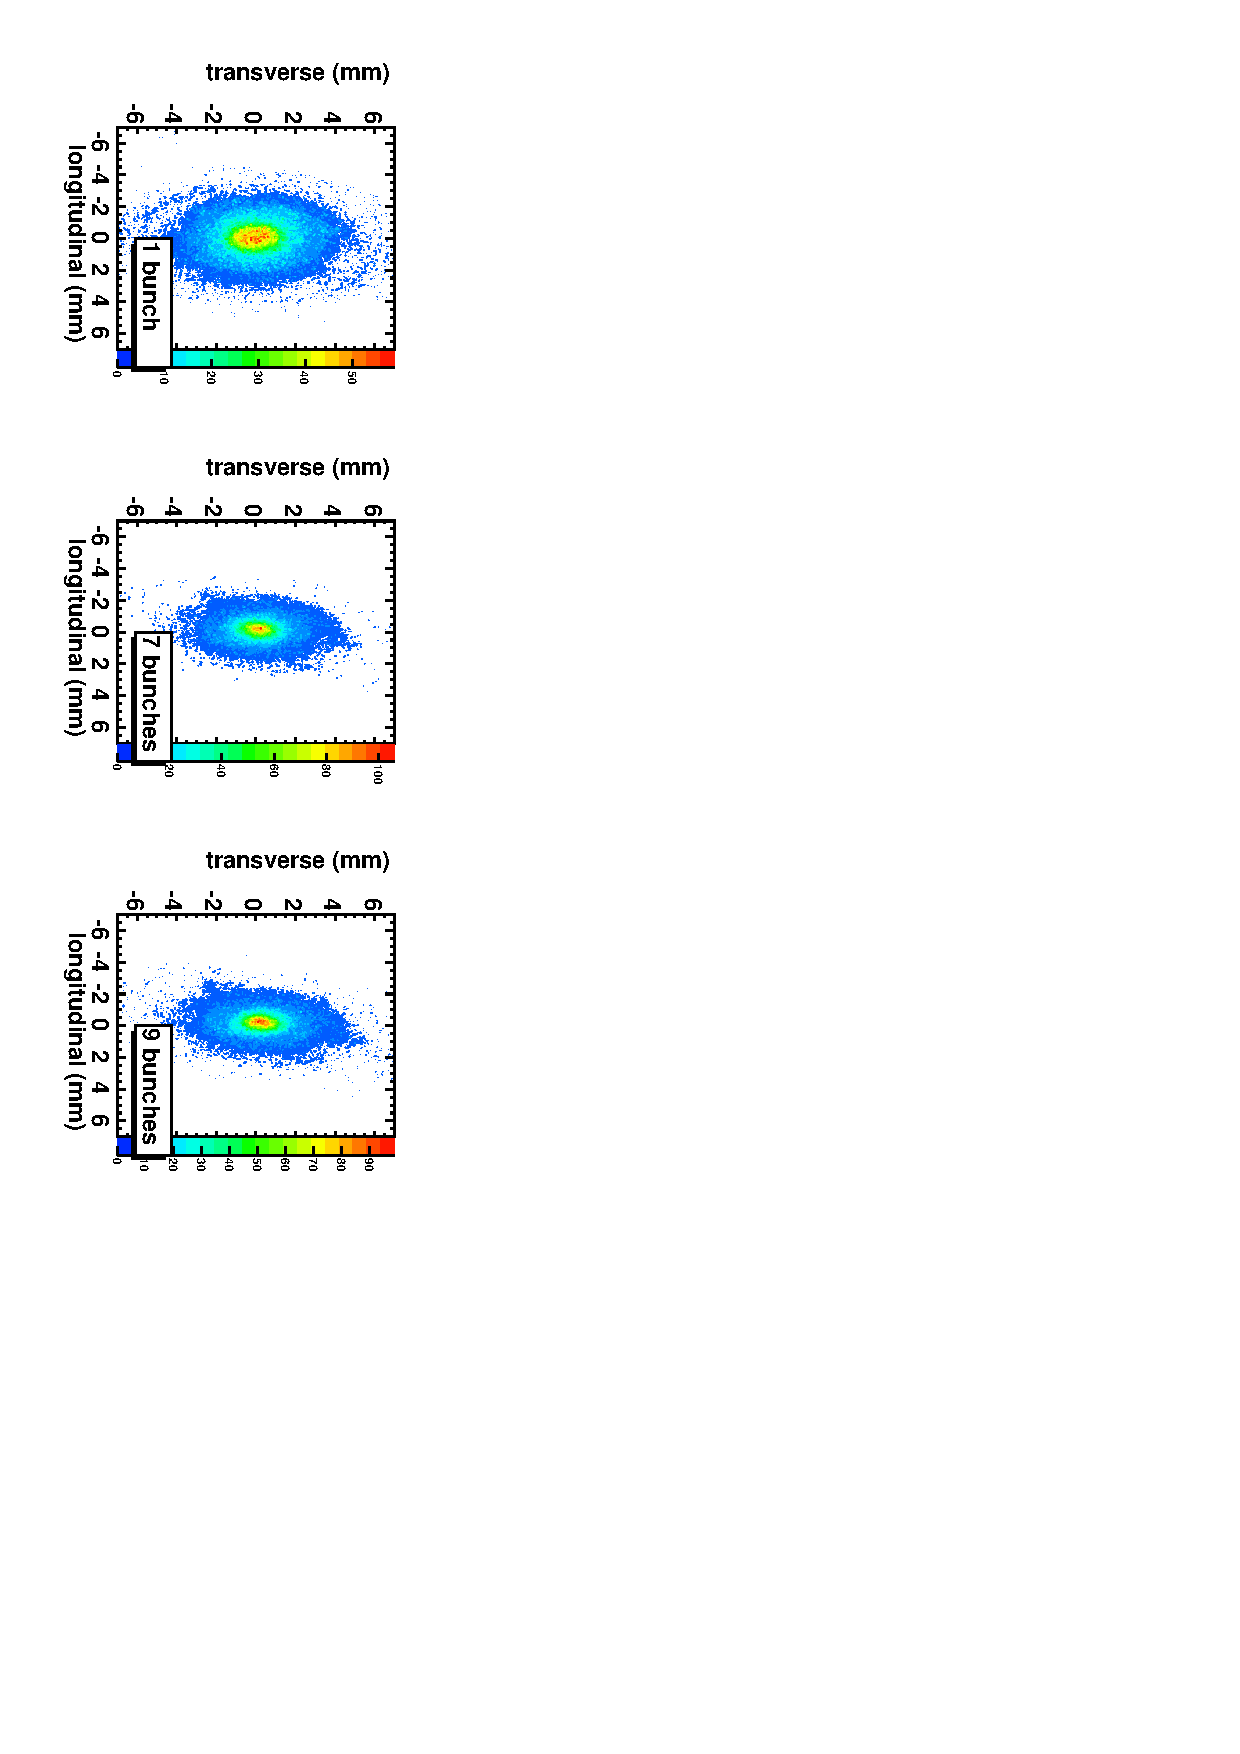
\includegraphics[angle=90,width=1.\textwidth]{figures/C9B7BSB-2D-1mA-80}
\end{center}
\end{figure}
\end{frame}

\begin{frame}{Figures-II}

\begin{figure}
\begin{center}
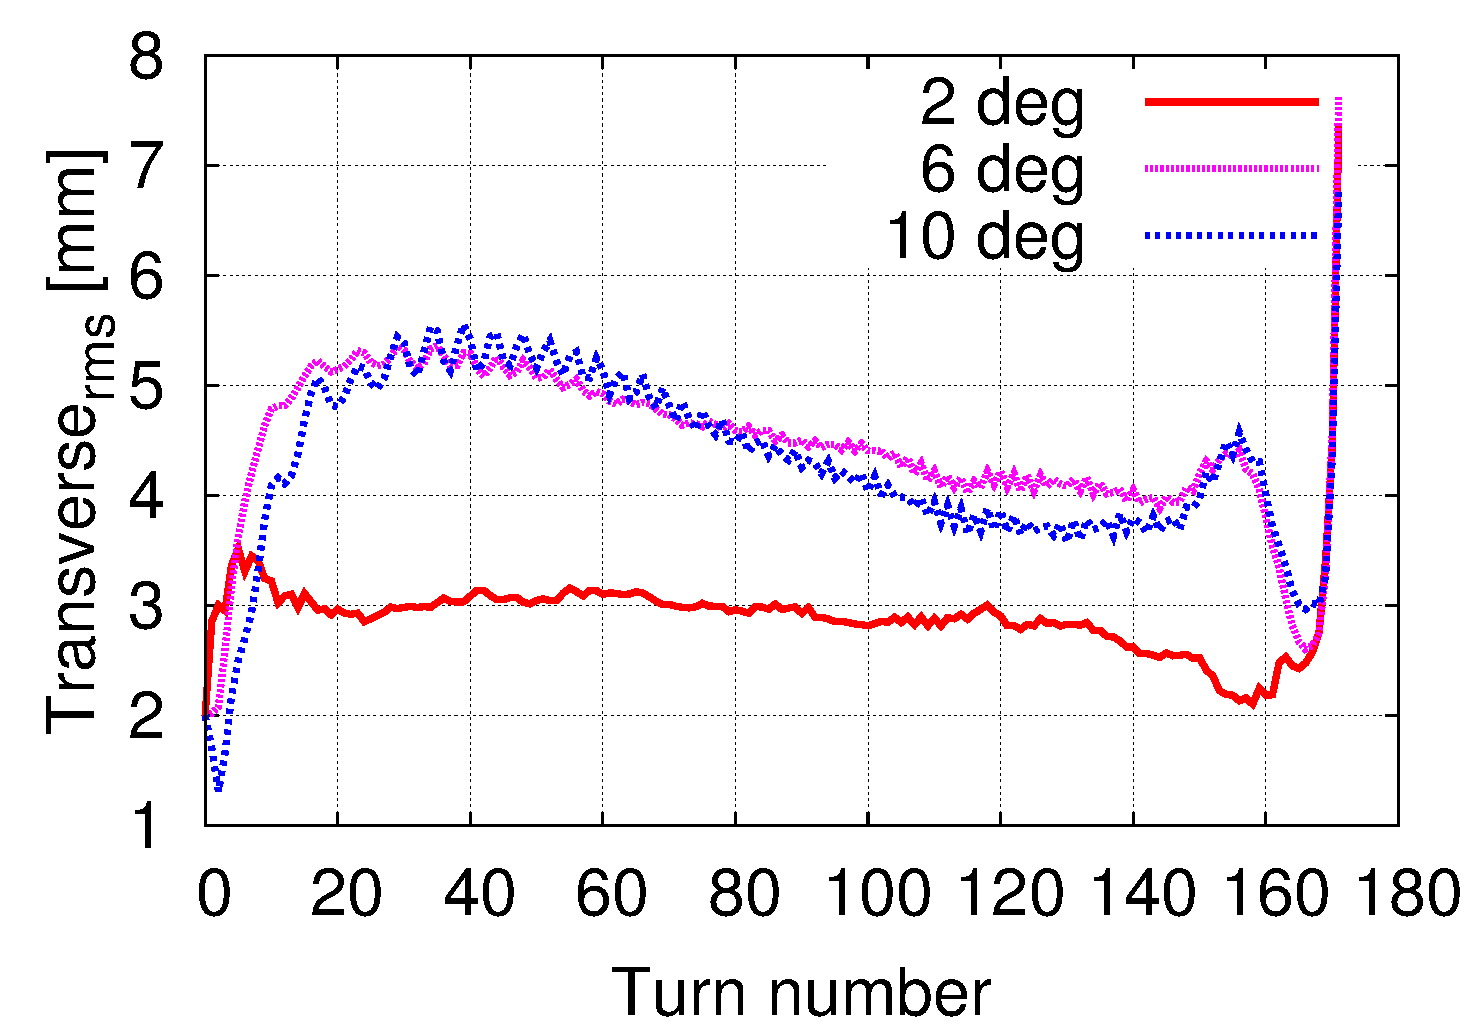
\includegraphics[angle=0,width=.9\textwidth]{figures/Comp-Transverse}
\end{center}
\end{figure}
\end{frame}

\begin{frame}[fragile]
  \frametitle{Example - Arrays}


  \begin{itemize}

      \item $\left\{
            \begin{array}{cccc}
              -\Delta u +\lambda u &= & |u|^{p-2}, &\textrm{ in } \Omega \\
              u &\geq & 0, & u\in H_0^1(\Omega)
            \end{array}
           \right.$


     \vfill

     \pause

     \item \begin{verbatim}
$\left\{
  \begin{array}{cccc}
  -\Delta u +\lambda u &= & |u|^{p-2}, &\textrm{ in }
  \Omega \\
  u &\geq & 0, & u\in H_0^1(\Omega)
  \end{array}
\right.$

\end{verbatim}

  \end{itemize}

\end{frame}


\begin{frame}[fragile]
  \frametitle{Example - Arrays}
   \framesubtitle{Change centering}

  \begin{itemize}

    \item $\left\{
            \begin{array}{lcrr}
              -\Delta u +\lambda u &= & |u|^{p-2}, &\textrm{ in } \Omega \\
              u &\geq & 0, & u\in H_0^1(\Omega)
            \end{array}
           \right.$

     \vfill

     \pause

     \item \begin{verbatim}
$\left\{
  \begin{array}{lcrr}
  -\Delta u +\lambda u &= & |u|^{p-2}, &\textrm{ in }
  \Omega \\
  u &\geq & 0, & u\in H_0^1(\Omega)
  \end{array}
\right.$

\end{verbatim}

  \end{itemize}

\end{frame}

\begin{frame}[fragile]
  \frametitle{Example - Arrays}
   \framesubtitle{Change centering}

  \begin{itemize}


    \item $\left\{
            \begin{array}{rcll}
              -\Delta u +\lambda u &= & |u|^{p-2}, &\textrm{ in } \Omega \\
              u &\geq & 0, & u\in H_0^1(\Omega)
            \end{array}
           \right.$

     \vfill

     \pause

     \item \begin{verbatim}
$\left\{
  \begin{array}{rcll}
  -\Delta u +\lambda u &= & |u|^{p-2}, &\textrm{ in }
  \Omega \\
  u &\geq & 0, & u\in H_0^1(\Omega)
  \end{array}
\right.$

\end{verbatim}

  \end{itemize}

\end{frame}


\begin{frame}[fragile]
  \frametitle{More Examples}

  \begin{itemize}

    \item $\ds \varphi (u) = \int_{\Omega} \left[ \dfrac{\|\nabla u\|^2}{2} + \lambda\dfrac{u^2}{2} - \dfrac{(u^+)^p}{p}\right] d\mu $

     \vfill

     \pause

     \item \begin{verbatim}
$\ds \varphi (u) = \int_{\Omega} \left[
 \dfrac{\|\nabla u\|^2}{2} +
 \lambda\dfrac{u^2}{2} -
 \dfrac{(u^+)^p}{p} \right] d\mu $

\end{verbatim}

  \end{itemize}

\end{frame}


\begin{frame}[fragile]
  \frametitle{Even More Examples}

De Morgan's Law

  \begin{itemize}

    \item $\ds \left(\bigcup_{i=1}^{n} A_i\right)^c =
     \bigcap_{i=1}^n A_i^c$

     \vfill

     \pause

     \item \begin{verbatim}
$\ds \left(\bigcup_{i=1}^{n} A_i\right)^c =
     \bigcap_{i=1}^n A_i^c$
\end{verbatim}

     \vfill

     \pause

     \item $A\times B = \set{(a,b)|a\in A, b\in B}$

     \vfill

     \pause

     \item \begin{verbatim}
$A\times B = \set{(a,b)|a\in A, b\in B}$
\end{verbatim}


  \end{itemize}

\end{frame}

\begin{frame}[fragile]
  \frametitle{Equations}

  \begin{itemize}

\item Consider the equation of Energy below.

 \begin{equation}\label{eq:energy}
     E(u) = \int |\nabla u|^2 dx
 \end{equation}

This is how we refer to \eqref{eq:energy}.

\pause

\vfill

\item\begin{verbatim}
 \begin{equation}\label{eq:energy}
     E(u) = \int |\nabla u|^2 dx
 \end{equation}

This is how we refer to \eqref{eq:energy}.
\end{verbatim}

\end{itemize}

\end{frame}


\begin{frame}[fragile]
  \frametitle{Equations}

  \begin{itemize}

\item Consider the equation without a number below.

 \begin{equation}
     E(u) = \int |\nabla u|^2 dx \nonumber
 \end{equation}


\pause

\vfill

\item\begin{verbatim}
 \begin{equation}\label{eq:energy}
     E(u) = \int |\nabla u|^2 dx \nonumber
 \end{equation}
\end{verbatim}

\end{itemize}

\end{frame}


\begin{frame}[fragile]
  \frametitle{Equations}
   \framesubtitle{Tag an equation}
  \begin{itemize}

\item Consider the equation with a tag

 \begin{equation}\label{eq:energytag}
     E(u) = \int |\nabla u|^2 dx \tag{E}
 \end{equation}

 If $u$ is harmonic, \eqref{eq:energytag} is preserved.

\pause

\vfill

\item\begin{verbatim}
 \begin{equation}\label{eq:energytag}
     E(u) = \int |\nabla u|^2 dx \tag{E}
 \end{equation}

If $u$ is harmonic, \eqref{eq:energytag} is preserved.
\end{verbatim}

\end{itemize}

\end{frame}

\begin{frame}[fragile]
  \frametitle{Equations}
   \framesubtitle{a small proof}
  \begin{itemize}

\item Indeed,

 \begin{equation}
  \begin{split}
   \dfrac{d}{dt} E(u) & = 2 \int \langle\nabla u,\nabla u\rangle\\
   & = -2 \int\langle\Delta u,u\rangle = 0
  \end{split}
 \end{equation}

\pause

\vfill

\item The ``='' signs are aligned.

\vfill

\pause

\item Use \begin{verbatim} \begin{split} ... \end{split}
\end{verbatim}


\end{itemize}

\end{frame}


\begin{frame}[fragile]
  \frametitle{Equations}
   \framesubtitle{a small proof}
  \begin{itemize}

\item \begin{verbatim}
 \begin{equation}
  \begin{split}
   \dfrac{d}{dt} E(u) & = 2 \int \langle\nabla u,
                                 \nabla u\rangle\\
   & = -2 \int\langle\Delta u,u\rangle = 0
  \end{split}
 \end{equation}

\end{verbatim}


\end{itemize}

\end{frame}




\begin{frame}[fragile]
  \frametitle{Equations}
   \framesubtitle{in an array}
  \begin{itemize}

\item Consider the expression below

 \begin{equation}
  \begin{split}
   (a+b)^2 &  = (a+b)(a+b) \\
           &  = a^2 +2ab +b^2
   \end{split}
 \end{equation}


\pause

\vfill

\item\begin{verbatim}
 \begin{equation}
  \begin{split}
   (a+b)^2 &  = (a+b)(a+b) \\
           &  = a^2 +2ab +b^2
  \end{split}
 \end{equation}
\end{verbatim}

\end{itemize}

\end{frame}




\begin{frame}[fragile]
  \frametitle{Environments}

  In LaTeX, environments must match:

  \begin{itemize}

  \item\begin{verbatim}
  \begin{...}
  .
  .
  .
  \end{...}
  \end{verbatim}

  \pause

  \item \$ ...\$ $\to$ for math symbols

  \pause

  \item \verb|\[ ... \]| $\to$ for centering expressions

  \pause

  \item \verb|\left( ... \right)| $\to$ match size of parentheses

  \end{itemize}

\end{frame}


\begin{frame}[fragile]
  \frametitle{Environments}
   \framesubtitle{delimiters}
  \begin{itemize}

  \item $(\ds\int|\nabla u|^p d\mu)^p$ versus $\left(\ds\int|\nabla u|^p d\mu\right)^p$

  \pause

  \vfill

  \item \begin{verbatim}
$(\ds\int|\nabla u|^p d\mu)^p$
  \end{verbatim}


  \item \begin{verbatim}
$\left(\ds\int|\nabla u|^p d\mu\right)^p$
  \end{verbatim}



\end{itemize}

\end{frame}




\begin{frame}[fragile]
  \frametitle{Tables}

  Consider the truth table:

  \jl

  \begin{tabular}{c c c | c}
$P$ & $Q$ & $\neg P$ & $\neg P\to (P \vee Q)$ \\ \hline
T & T & F & T \\
T & F & F & T \\
F & T & T & T \\
F & F & T & F
\end{tabular}


\end{frame}


\begin{frame}[fragile]
  \frametitle{Tables - code}
\begin{verbatim}

  \begin{tabular}{c c c | c}
$P$ & $Q$ & $\neg P$ & $\neg P\to (P \vee Q)$ \\ \hline
T & T & F & T \\
T & F & F & T \\
F & T & T & T \\
F & F & T & F

\end{tabular}

\end{verbatim}


\end{frame}
\end{comment}


\begin{frame}
\vspace{-3mm}  
\frametitle{References}
%\begin{thebibliography}{99} 
%\bibitem[J. Yang, A. Adelmann, et al., NIM-A {\bf 704}(11) (2013)] {daeiso} J. Yang, Adelmann et al.,  NIM-A {\bf 704}(11) 84-91 (2013)
%\bibitem[J. M. Conrad, M. H. Shaevitz PRL {\bf104}, 141802 (2010)]{daed}J. M. Conrad, M. H. Shaevitz, Multiple Cyclotron Method to Search for CP Violation in the Neutrino Sector Phys. Rev. Lett. {\bf104}, 141802 (2010)
%\bibitem[A. Adelmann et al. arXiv:1207.4895]{daednim}Multimegawatt DAE$\delta$ALUS Cyclotrons for Neutrino Physics, A. Adelmann et al., arXiv:1207.4895 [physics.acc-ph]
%\bibitem[M. Toggweiler et al., arXiv:1211.3664 (2012), submitted JCP]{TM} M. Toggweiler, A. Adelmann, P. Arbenz, J.J. Yang, arXiv:1211.3664 (2012)
%\end{thebibliography}
\printbibliography
\end{frame}
\end{document}